\chapter{Descripción de la Misión}
El proyecto ha sido nombrado LAMBDA, acrónimo de LAMBDA Analyzes Microorganisms' Damage in
Anomalous Conditions. Este nombre resume el propósito principal de la misión: analizar la
viabilidad de células eucariotas expuestas a las condiciones extremas del vuelo del CubeSat.

En este capítulo se detallan los objetivos y requerimientos de las dos misiones que conforman el
proyecto:
la misión primaria, impuesta por la competencia, y la misión secundaria, desarrollada en
colaboración con el Instituto de Investigación Médica Mercedes y Martín Ferreyra (INIMEC-CONICET
UNC).

Se describe técnicamente el CubeSat encargado de llevar a cabo ambas misiones, incluyendo todos
los subsistemas necesarios para su operación, así como los presupuestos de masa, potencia y datos.
Finalmente, se enumeran los ensayos a los que será sometido durante el desarrollo para validar
los conceptos desarrollados.

Además, se presenta un plan de proyecto que detalla la organización del equipo para cumplir con
los requerimientos de la competencia.

\section{Objetivos Misión Primaria}
La misión principal del presente proyecto consiste en registrar durante todo el vuelo del
CubeSat ciertas variables físicas, las cuales son:

  \begin{itemize}
    \item Presión atmosférica,
    \item Temperatura ambiente,
    \item Aceleración en los tres ejes,
    \item Angulo de giro en los tres ejes.
  \end{itemize}

Estas mediciones serán recopiladas, filtradas y almacenadas, y permitirán llevar a cabo
diversos análisis sobre el comportamiento del CubeSat durante su vuelo.

El objetivo será aprovechar dichas mediciones para determinar el instante en el que se
alcanza el apogeo y su altitud máxima (valor de apogeo) respecto al punto de lanzamiento.
Por otro lado, también se determinará el tiempo total de ascenso y descenso, y se identificarán
las distintas fases del vuelo, tales como: inicio del ascenso, fin de la propulsión, el apogeo,
y finalmente, la recuperación.

Estas determinaciones, ademas de cumplir con los requisitos mínimos establecidos por la
organización de la competencia, serán de gran utilidad para la misión secundaria propuesta,
ya que permitirán interpretar correctamente los resultados obtenidos de la experimentación
a realizar, que será detallada en la siguiente sección.

\section{Objetivos Misión Secundaria}
  \subsection{General}
    La misión secundaria del CubeSat, desarrollada en colaboración con el Instituto de Investigación
    Medica Mercedes y Martín Ferreyra (INIMEC-CONICET-UNC).

    En el Laboratorio de Microbiología del Instituto M y M Ferreyra-INIMEC-UNC, se estudia desde hace más de 20 años
    distintos aspectos de la biología celular y molecular del parásito Giardia Lamblia, en condiciones óptimas de
    cultivo. El experimento planteado tiene como propósito estudiar las respuestas fisiológicas y cambios moleculares
    de este parásito luego de su exposición a condiciones extremas simuladas de altura, como paso preliminar para
    evaluar su potencial resistencia a entornos hostiles y comprender su plasticidad celular.

    Los principales entornos hostiles incluyen las vibraciones mecánicas y
    las aceleraciones experimentadas durante el trayecto. Para ello, se analizaran varias muestras
    celulares dispuestas en condiciones experimentales distintas, con el objetivo de identificar
    posibles diferencias en sus respuestas fisiológicas.

    El sistema contara con control térmico tanto para mantener la temperatura dentro de
    un rango adecuado para la preservación celular, como para someter distintas muestras a
    distintas condiciones de temperatura. Posteriormente, se llevara a cabo un análisis post vuelo a
    fin de evaluar los efectos del entorno sobre cada muestra, mediante la observación de
    cambios estructurales o alteraciones morfológicas en las células.


  \subsection{Giardia Lamblia}
    La \textit{Giardia Lamblia} es un protozoario parásito flagelado que coloniza el intestino humano
    y animal, siendo una causa muy frecuente de enfermedad intestinal, contribuyendo a la carga
    de malnutrición en todo el mundo. La enfermedad producida por este parásito conocida
    como giardiasis es una parasitosis con gran importancia clínica y epidemiológica. Siendo esta
    la infección parasitaria del intestino humano mas frecuente de todo el mundo.

    Una característica importante que poseen los microorganismos parásitos es su gran capacidad de
    adaptación a los cambios del medio ambiente. La mayoría de los parásitos ocupan
    diferentes nichos durante su travesa a por vectores y huéspedes, desarrollando extraordinarios
    mecanismos de adaptación que les permiten sobrevivir en condiciones que de otro modo
    los destruirán. Particularmente, \textit{Giardia Lamblia} experimenta un proceso de diferenciación
    a quiste, conocido como enquistamiento \cite{gda}.

    El ciclo de vida simple de dos etapas de \textit{Giardia} es central para su éxito como parásito. Los
    quistes de \textit{Giardia Lamblia} pueden sobrevivir en agua dulce fría durante meses, y se necesitan
    menos de 10 quistes para la infección humana. La exposición de los quistes ingeridos al ácido
    gástrico desencadena el desenquistamiento, una diferenciación rápida y dramática.

    Después de la entrada en el intestino delgado, la pared del quiste se abre y emerge el
    parásito. Los \textit{trofozoítos} colonizan por debajo de la entrada del conducto biliar común y pueden
    causar enfermedades, aunque no invaden. Si son transportados rió abajo, los \textit{trofozoítos}
    deben enquistarse para sobrevivir fuera del huésped. In vitro, \textit{Giardia} se enquista en respuesta a
    los estímulos fisiológicos de aumento de bilis y pH ligeramente alcalino [2]. El estándar
    de oro para una enquistación exitosa es la capacidad de los quistes para desenquistarse.

    Otros parásitos intestinales importantes, como \textit{Entamoeba}, \textit{Toxoplasma}, \textit{Cryptosporidium}, varias
    \textit{tenias} y \textit{nematodos}, se transmiten en forma de quistes u ooquistes. Sin embargo,
    el estudio de estos organismos se ve limitado por la imposibilidad de generar quistes maduros
    in vitro a diferencia de la \textit{Giardia Lamblia}, por lo que se considera a este como un modelo
    de estudio para los demás parásitos.

    La vía de enquistamiento de \textit{Giardia} es un mecanismo clave de virulencia cuyo objetivo
    biológico es la diferenciación hacia una forma que pueda sobrevivir en el ambiente e infectar
    a un nuevo huésped. El enquistamiento también promueve la evasión inmunitaria y es un
    objetivo para el desarrollo de vacunas y fármacos.

    La desenquistación es una transformación gradual
    del \textit{trofozoíto} móvil, flagelado, binucleado y con forma de media pera (Figura \ref{fig:enquistamiento}).
    Los \textit{trofozoítos} pierden su capacidad de fijación a la pared intestinal; los fragmentos del disco de
    fijación y los flagelos se internalizan. El metabolismo también disminuye a medida que las células
    se redondean y entran en latencia.

    \begin{figure}[H]
      \centering
      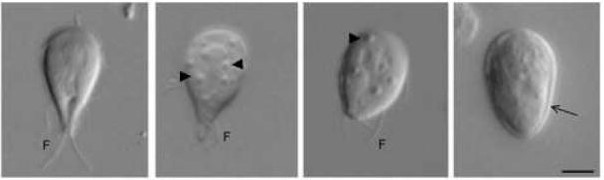
\includegraphics[width=1\textwidth]{./image/Giardia/Enquistamiento.jpg}
      \caption{Enquistamiento de \textit{Giardia Lamblia}: del trofozoíto al quiste. F, flagelos. Barra: 5 $\mu m$}
      \label{fig:enquistamiento}
    \end{figure}

    Las imágenes de izquierda a derecha muestran un trofozoíto vegetativo, trofozoítos después de 21 y
    42 horas de enquistamiento y un quiste resistente al agua. \cite{Lauwaet2007-te}

  \subsection{Experimento}
    Se establecieron tres condiciones experimentales con el objetivo de evaluar el efecto de las
    variables asociadas al lanzamiento sobre el crecimiento y viabilidad de las muestras biológicas.
    Las condiciones diseñadas son las siguientes:
 
    \begin{itemize}
      \item \textbf{Condición de vuelo (CubeSat):} las muestras serán enviadas a bordo del CubeSat y
      sometidas a diferentes temperaturas: $10\Celsius$, $37\Celsius$ (considerada óptima para el
      crecimiento) y $55\Celsius$. Adicionalmente, se incluirá una muestra sin control activo de temperatura,
      expuesta a las variaciones térmicas propias del entorno.

      Todas las capsulas estarán posicionadas con una inclinación de 45 con respecto al eje horizontal, condición
      necesaria para favorecer la adherencia del parásito al medio de cultivo. Se busca analizar el
      impacto combinado de la micro gravedad, las variaciones de presión, aceleraciones
      y la exposición térmica.

      \item \textbf{Condición control terrestre (estación terrestre):} se replicará en tierra
      el mismo diseño experimental térmico y la misma orientación espacial de las capsulas
      que en el CubeSat. No obstante, las muestras permanecerán en un entorno terrestre
      controlado, sin estar expuestas a los factores propios del vuelo. Esta condición permitirá
      distinguir los efectos del lanzamiento de aquellos debidos a la condición térmica
      aplicada.

      \item \textbf{Condición control optima (laboratorio):} se cultivará una muestra en condiciones optimas
      conocidas para el organismo en estudio: temperatura constante de
      $37\Celsius$, capsula inclinada a 45 y en ausencia de movimiento. Esta condición constituye
      el control biológico para el experimento y servirá como referencia para evaluar posibles
      desviaciones en las demás muestras.

      En todos los casos, se mantendrán constantes el tipo de recipiente utilizado, el medio de cultivo y la cantidad
      inicial de trofozoítos inoculados por
      capsula. Asimismo, tanto las muestras de las condiciones a) como b) serán sometidas al mismo
      proceso de traslado previo al inicio del experimento, con el fin de asegurar homogeneidad en
      las condiciones iniciales.
    \end{itemize}

  \subsection{Ensayos}
    Se realizarán ensayos a posteriori para evaluar si las condiciones a las cuales fue sometido afectaron la
    viabilidad o si las situaciones de estrés disparan mecanismos clásicos de adaptación de Giardia Lamblia, como por
    ejemplo; el enquistamiento, procesos de apoptosis, etcétera.

    Para ello se cultivarán los trofozoítos en un medio líquido, en condiciones de anaerobiosis a 37°C, en medio
    TYI-S-33 (pH 7) suplementado con 10\% de suero bovino adulto y 5\% de bilis bovina (medio completo de crecimiento).
    El día del comienzo de la misión se analizará viabilidad celular utilizando trypan blue (colorante que colorea
    células muertas) y se colocará la misma cantidad de trofozoítos en las tres condiciones (cubesat, estación
    terrestre y laboratorio), en iguales recipientes (cápsulas).

    Para analizar los genes asociados a la respuesta al estrés, al finalizar el experimento, se extraerá ARN (ácido
    ribonucleico) de las tres muestras, se sintetizará cDNA y luego se cuantificará por medio de real-time PCR (qPCR)
    genes asociados al estrés (por ej. HSP70, proteínas de choque térmico, oxidorreductasas, etc). Se utilizará GDH
    como gen constitutivo y se analizará si se observan cambios en las muestras en las condiciones planteadas con
    respecto al cultivo crecido en el laboratorio.

    Para hacer un análisis del proceso de enquistamiento, debido a que el sometimiento del parásito a situaciones de
    estrés desencadena el proceso de enquistamiento proponemos obtener las muestras luego de finalizar el experimento
    y analizar por medio de ensayos de inmunofluorescencia si se expresan las proteínas asociadas al proceso de
    enquistamiento. Para ello fijaremos las células, realizaremos los ensayos de inmunofluorescencia, y posteriormente
    las observaremos utilizando microscopía de fluorescencia. Se analizará si bajo estas circunstancias particulares se
    evidencian vesículas específicas de enquistamiento, un signo adicional de estrés celular.

  \subsection{Procedimientos}
    Esta sección describe los procedimientos necesarios para el cultivo y traslado de las muestras
    biológicas utilizadas en el experimento, manteniendo condiciones estandarizadas que
    aseguren su viabilidad y reproducibilidad.

    \subsubsection{Cultivo}
    Para cultivarloLauwaet2007-tes axenicamente se utiliza medio TYI-S-33 (pH 7) suplementado con 10\% de
    suero bovino adulto y 5\% de bilis bovina (medio completo de crecimiento) (Diamond, Harlow
    un volumen determinado de medio. Los tubos se colocaron en gradillas orientadas con una
    inclinación de aproximadamente $45\degree$, dentro de una estufa de cultivo a $37 \Celsius$.

    Luego de una hora, se comienza a observar la adhesión de los trofozoítos a las paredes del
    tubo a través de su disco ventral. De esta manera, se reproduce un entorno similar al que se
    encuentra in vivo, permitiendo la división de los trofozoítos. A las 48 horas se obtiene una
    mono-capa de trofozoítos en etapa de crecimiento. La inclinación de las gradillas favorece
    una mayor superficie de adhesión sobre las paredes del tubo.

    \subsubsection{Traslado}
    Las condiciones optimas para el traslado consisten en mantener las muestras a $37\Celsius$ y con
    una inclinación de $45\degree$. El tiempo de traslado puede extenderse hasta 48 horas sin que esto
    afecte significativamente las condiciones de crecimiento del parásito.

\section{Descripción del CubeSat}
En esta sección se presenta una descripción técnica del CubeSat diseñado para llevar a
cabo las misiones planteadas previamente. Se detallara como se planea abordar la implementación de
los objetivos definidos, a través de la integración de subsistemas electrónicos, mecánicos y de software.

Se incluyen diagramas de bloques que representan la arquitectura general del sistema y la
interacción entre los distintos subsistemas, tales como adquisición de datos, almacenamiento,
alimentación eléctrica y control de sensores. Asimismo, se describen las herramientas de
calculo y simulación empleadas durante las etapas de diseño y verificación preliminar.

También se presentan estimaciones iniciales de los presupuestos de masa, consumo de
potencia y volumen de datos, los cuales resultan fundamentales para validar la viabilidad del
sistema dentro de las restricciones impuestas por la competencia.

El desarrollo de esta sección tiene por objetivo demostrar la coherencia técnica entre los
requerimientos de misión y el diseño propuesto, as como documentar las decisiones adoptadas
durante el proceso de ingeniera del CubeSat.

  \subsection{General}
    En la Figura 5.2 se presenta el diagrama en bloques del sistema general desarrollado para
    el proyecto. El sistema general permite integrar la misión principal, enfocada en la recolección
    de parámetros ambientales, con una misión secundaria orientada al control y documentación de
    las condiciones de las muestras transportadas.

    \begin{figure}[H]
      \centering
      \resizebox{\textwidth}{!}{
      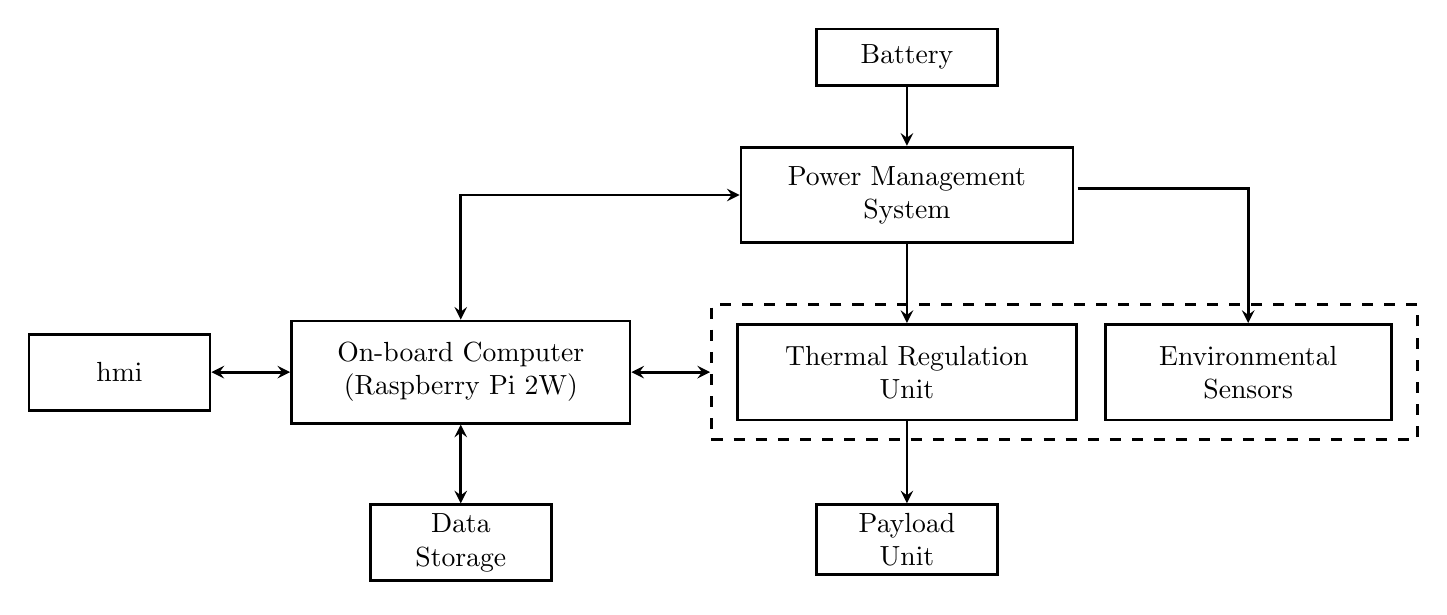
\begin{tikzpicture}
        % Paths, nodes and wires:
        \node[shape=rectangle, draw, line width=1pt, dash pattern={on 4pt off 4pt}, inner sep=0, minimum width=8.965cm, minimum height=1.715cm] at (11.833, 1.333){};
        \node[shape=rectangle, draw, line width=1pt, inner sep=0, minimum width=4.298cm, minimum height=1.215cm] at (9.833, 1.333){} node [anchor=center, align=center, text width=3.91cm, inner sep=5.5pt] at (9.833, 1.333){Thermal Regulation\\Unit};
        \node[shape=rectangle, draw, line width=1pt, inner sep=0, minimum width=3.631cm, minimum height=1.215cm] at (14.167, 1.333){} node [anchor=center, align=center, text width=3.243cm, inner sep=5.5pt] at (14.167, 1.333){Environmental Sensors};
        \node[shape=rectangle, draw, line width=1pt, inner sep=0, minimum width=2.298cm, minimum height=0.881cm] at (9.833, -0.792){} node [anchor=center, align=center, text width=1.91cm, inner sep=5.5pt] at (9.833, -0.792){Payload Unit};
        \node[shape=rectangle, draw, line width=1pt, inner sep=0, minimum width=2.298cm, minimum height=0.965cm] at (4.167, -0.833){} node [anchor=center, align=center, text width=1.91cm, inner sep=5.5pt] at (4.167, -0.833){Data Storage};
        \node[shape=rectangle, draw, line width=1pt, inner sep=0, minimum width=2.298cm, minimum height=0.715cm] at (9.833, 5.333){} node [anchor=center, align=center, text width=1.91cm, inner sep=5.5pt] at (9.833, 5.333){Battery};
        \node[shape=rectangle, draw, line width=1pt, inner sep=0, minimum width=4.298cm, minimum height=1.298cm] at (4.167, 1.333){} node [anchor=center, align=center, text width=3.91cm, inner sep=5.5pt] at (4.167, 1.333){On-board Computer\\(Raspberry Pi 2W)};
        \node[shape=rectangle, draw, line width=1pt, inner sep=0, minimum width=4.215cm, minimum height=1.215cm] at (9.833, 3.583){} node [anchor=center, align=center, text width=3.827cm, inner sep=5.5pt] at (9.833, 3.583){Power Management\\System};
        \draw[stealth-stealth, line width=1pt] (4.167, 2) |- (7.708, 3.583);
        \draw[-stealth, line width=1pt] (12, 3.667) -| (14.167, 1.958);
        \draw[stealth-, line width=1pt] (9.833, 4.208) -- (9.833, 4.958);
        \draw[stealth-, line width=1pt] (9.833, 1.958) -- (9.833, 2.958);
        \draw[stealth-stealth, line width=1pt] (4.167, 0.667) -- (4.167, -0.333);
        \node[shape=rectangle, draw, line width=1pt, inner sep=0, minimum width=2.298cm, minimum height=0.965cm] at (-0.167, 1.333){} node [anchor=center, align=center, text width=1.91cm, inner sep=5.5pt] at (-0.167, 1.333){\acrshort{hmi}};
        \draw[stealth-, line width=1pt] (9.833, -0.333) |- (9.833, 0.708);
        \draw[stealth-stealth, line width=1pt] (7.333, 1.333) -- (6.333, 1.333);
        \draw[stealth-stealth, line width=1pt] (1, 1.333) -- (2, 1.333);
      \end{tikzpicture}
      }
      \caption{Diagrama en bloques del sistema general}
      \label{fig:sistema_general}
    \end{figure}

  \subsection{Descripción de Subsistemas}
    A continuación, se describe la función de cada bloque y su interacción dentro del sistema:
    \begin{itemize}
      \item \textbf{Battery:} Se emplearan seis baterías de pollero de litio (Li-Po) con una tensión nominal de 3.7V
      y una capacidad individual de 3200mAh. Estas se organizaran en tres ramas
      conectadas en paralelo, cada una conformada por dos baterías en serie. Esta configuración proporciona una tensión total de 7.4V por rama (suma de dos baterías de 3.7V en
      serie) y una capacidad total de 71.04Wh, adecuada para satisfacer los requerimientos
      energéticos del CubeSat durante su operación.

      \item \textbf{\acrfull{pms}:} es el subsistema responsable de administrar
      de forma segura y eficiente la energía proveniente de las baterías o de una fuente externa. Su función principal es
      distribuir la energía eléctrica a los distintos subsistemas del CubeSat, garantizando condiciones adecuadas de operación, mediante el monitoreo, la protección y la regulación.
      Específicamente, las funciones del \acrshort{pms} son:
      \begin{itemize}
        \item Proteger contra cortocircuitos o sobrecarga de corriente,
        \item Permite medir parámetros eléctricos (como tensión y corriente) y gestionar el
          encendido y apagado selectivo de distintos rieles de alimentación lo que contribuye
          a una mejor eficiencia energética y diagnostico en vuelo,
        \item Generar y estabilizar distintos niveles de tensión requeridos por los subsistemas
          del CubeSat, como 3.3V para sensores, 5V para la computadora de abordo y 12V
          para cargas especificas.
      \end{itemize}

      Con la finalidad de disminuir la carga en las baterías, se suministrará energía al \acrshort{pms} por medio de una fuente de
      alimentación externa durante la fase inicial del control de temperatura ya que este es momento donde las celdas
      de Peltier demandan mayor cantidad de energía, drenando rápidamente la carga de las baterías. Al llegar a las
      temperaturas deseadas, ya la demanda de energía es mucho menor, posibilitando la desconexión de la fuente externa sin
      perjudicar la autonomía del CubeSat.

      En definitiva, el \acrshort{pms} asegura que los requerimientos energéticos del CubeSat sean
      satisfechos de manera controlada, segura y adaptable durante toda la misión.

      \begin{figure}[H]
        \centering
        \resizebox{130mm}{!}{
        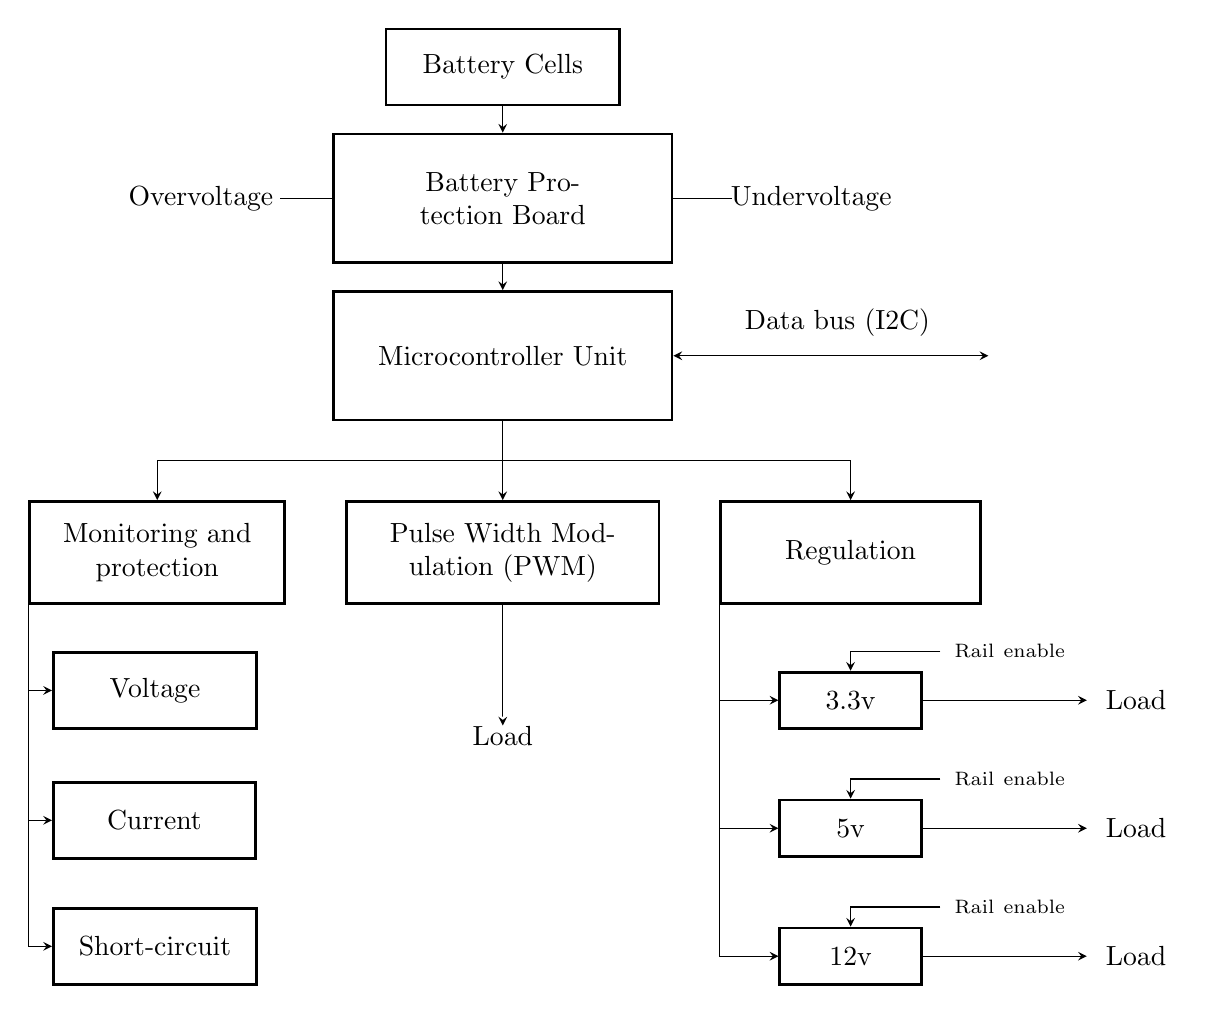
\begin{tikzpicture}
            % Paths, nodes and wires:
            \node[shape=rectangle, draw, line width=1pt, inner sep=0, minimum width=2.965cm, minimum height=0.965cm] at (8.5, 11.5){} node [anchor=center, align=center, text width=2.577cm, inner sep=5.5pt] at (8.5, 11.5){Battery Cells};
            \node[shape=rectangle, draw, line width=1pt, inner sep=0, minimum width=4.298cm, minimum height=1.631cm] at (8.5, 7.833){} node [anchor=center, align=center, text width=3.91cm, inner sep=5.5pt] at (8.5, 7.833){Microcontroller Unit\\};
            \node[shape=rectangle, draw, line width=1pt, inner sep=0, minimum width=4.298cm, minimum height=1.631cm] at (8.5, 9.833){} node [anchor=center, align=center, text width=3.91cm, inner sep=5.5pt] at (8.5, 9.833){Battery Protection Board};
            \node[shape=rectangle, inner sep=0, minimum width=2.5cm, minimum height=1cm] at (4.667, 9.833){} node [anchor=center, align=center, text width=2.147cm, inner sep=5pt] at (4.667, 9.833){Overvoltage};
            \node[shape=rectangle, draw, line width=1pt, inner sep=0, minimum width=3.24cm, minimum height=1.298cm] at (4.112, 5.333){} node [anchor=center, align=center, text width=2.852cm, inner sep=5.5pt] at (4.112, 5.333){Monitoring and\\protection\\};
            \node[shape=rectangle, draw, line width=1pt, inner sep=0, minimum width=1.798cm, minimum height=0.715cm] at (12.917, 3.458){} node [anchor=center, align=center, text width=1.41cm, inner sep=5.5pt] at (12.917, 3.458){3.3v};
            \node[shape=rectangle, draw, line width=1pt, inner sep=0, minimum width=3.298cm, minimum height=1.298cm] at (12.917, 5.333){} node [anchor=center, align=center, text width=2.91cm, inner sep=5.5pt] at (12.917, 5.333){Regulation\\};
            \node[shape=rectangle, draw, line width=1pt, inner sep=0, minimum width=2.581cm, minimum height=0.965cm] at (4.083, 0.333){} node [anchor=center, align=center, text width=2.193cm, inner sep=5.5pt] at (4.083, 0.333){Short-circuit};
            \draw[-stealth] (8.5, 9) -| (8.5, 8.667);
            \draw[-stealth] (8.5, 11) -| (8.5, 10.667);
            \draw[-stealth] (13.833, 3.458) -- (15.917, 3.458);
            \draw[stealth-stealth] (10.667, 7.833) -- (14.667, 7.833);
            \node[shape=rectangle, draw, line width=1pt, inner sep=0, minimum width=2.581cm, minimum height=0.965cm] at (4.083, 3.583){} node [anchor=center, align=center, text width=2.193cm, inner sep=5.5pt] at (4.083, 3.583){Voltage};
            \node[shape=rectangle, inner sep=0, minimum width=3.333cm, minimum height=0.667cm] at (12.75, 8.25){} node [anchor=center, align=center, text width=2.981cm, inner sep=5pt] at (12.75, 8.25){Data bus (I2C)};
            \node[shape=rectangle, inner sep=0, minimum width=2.5cm, minimum height=1cm] at (12.417, 9.833){} node [anchor=center, align=center, text width=2.147cm, inner sep=5pt] at (12.417, 9.833){Undervoltage};
            \draw (6.333, 9.833) -| (5.667, 9.833);
            \draw (10.667, 9.833) -- (11.417, 9.833);
            \node[shape=rectangle, draw, line width=1pt, inner sep=0, minimum width=2.565cm, minimum height=0.965cm] at (4.075, 1.933){} node [anchor=center, align=center, text width=2.177cm, inner sep=5.5pt] at (4.075, 1.933){Current};
            \node[shape=rectangle, inner sep=0, minimum width=2.063cm, minimum height=0.5cm] at (15.087, 4.083){} node [anchor=west, align=left, text width=1.71cm, inner sep=5pt] at (14.056, 4.083){\scriptsize Rail enable};
            \draw[-stealth] (14.056, 4.083) -| (12.917, 3.833);
            \node[shape=rectangle, draw, line width=1pt, inner sep=0, minimum width=1.798cm, minimum height=0.715cm] at (12.917, 1.833){} node [anchor=center, align=center, text width=1.41cm, inner sep=5.5pt] at (12.917, 1.833){5v};
            \draw[-stealth] (13.833, 1.833) -- (15.917, 1.833);
            \node[shape=rectangle, inner sep=0, minimum width=2.063cm, minimum height=0.5cm] at (15.087, 2.458){} node [anchor=west, align=left, text width=1.71cm, inner sep=5pt] at (14.056, 2.458){\scriptsize Rail enable};
            \draw[-stealth] (14.056, 2.458) -| (12.917, 2.208);
            \node[shape=rectangle, draw, line width=1pt, inner sep=0, minimum width=1.798cm, minimum height=0.715cm] at (12.917, 0.208){} node [anchor=center, align=center, text width=1.41cm, inner sep=5.5pt] at (12.917, 0.208){12v};
            \draw[-stealth] (13.833, 0.208) -- (15.917, 0.208);
            \node[shape=rectangle, inner sep=0, minimum width=2.063cm, minimum height=0.5cm] at (15.087, 0.833){} node [anchor=west, align=left, text width=1.71cm, inner sep=5pt] at (14.056, 0.833){\scriptsize Rail enable};
            \draw[-stealth] (14.056, 0.833) -| (12.917, 0.583);
            \draw[-stealth] (11.25, 4.667) |- (12, 0.208);
            \draw[stealth-] (12, 1.833) -| (11.247, 1.829);
            \draw[stealth-] (12, 3.458) -| (11.252, 3.461);
            \draw[-stealth] (2.475, 4.667) |- (2.775, 0.333);
            \draw[stealth-] (2.775, 3.583) -| (2.473, 3.591);
            \draw[stealth-] (2.775, 1.933) -| (2.474, 1.94);
            \node[shape=rectangle, draw, line width=1pt, inner sep=0, minimum width=3.965cm, minimum height=1.298cm] at (8.5, 5.333){} node [anchor=center, align=center, text width=3.577cm, inner sep=5.5pt] at (8.5, 5.333){Pulse Width Modulation (PWM)\\};
            \node[shape=rectangle, inner sep=0, minimum width=1.25cm, minimum height=0.5cm] at (8.5, 3){} node [anchor=center, align=center, text width=0.897cm, inner sep=5pt] at (8.5, 3){Load};
            \draw[stealth reversed-] (8.5, 3.25) -| (8.5, 4.667);
            \node[shape=rectangle, inner sep=0, minimum width=1.25cm, minimum height=0.5cm] at (16.542, 3.458){} node [anchor=center, align=center, text width=0.897cm, inner sep=5pt] at (16.542, 3.458){Load};
            \node[shape=rectangle, inner sep=0, minimum width=1.25cm, minimum height=0.5cm] at (16.542, 1.833){} node [anchor=center, align=center, text width=0.897cm, inner sep=5pt] at (16.542, 1.833){Load};
            \node[shape=rectangle, inner sep=0, minimum width=1.25cm, minimum height=0.5cm] at (16.542, 0.208){} node [anchor=center, align=center, text width=0.897cm, inner sep=5pt] at (16.542, 0.208){Load};
            \draw[-stealth] (8.5, 7) -| (8.5, 6);
            \draw[stealth-] (4.112, 6) |- (8.5, 6.5);
            \draw[stealth-] (12.917, 6) |- (8.5, 6.5);
        \end{tikzpicture}
        }
        \caption{Diagrama en bloques del subsistema \acrfull{pms}.}
        \label{fig:sistema_pms}
      \end{figure}

      \item \textbf{On-board Computer (\acrshort{obc}):} Tiene como función principal la gestión autónoma de
        la misión durante todo el vuelo. Esta unidad esta basada en una Raspberry Pi Zero 2
        W, equipada con el sistema operativo Raspberry Pi OS Lite, una versión optimizada sin
        entorno gráfico. Esta configuración fue seleccionada por su bajo consumo energético,
        reducido tamaño y alta estabilidad operativa, cualidades esenciales para sistemas embarcados
        en entornos aeroespaciales.

        El propósito fundamental del \acrshort{obc} es tomar y almacenar el registro de los sensores,
        tales como aceleración, orientación, presión atmosférica y temperatura ambiente. Estas
        mediciones son gestionadas por el firmware, y almacenadas de forma estructurada
        facilitando su posterior lectura y procesamiento.

        El \acrshort{obc} también es responsable del control de subsistemas clave, como el de regulación
        térmica, utilizado para la misión secundaria mediante celdas Peltier, a través del Sistema de
        administración de energía (\acrshort{pms}) y la lectura de los sensores ambientales. Ademas, mantiene una
        constante conexión con este sistema, actuando como intermediario entre el \acrshort{pms} y el \acrshort{hmi}, lo
        que permite el monitoreo en tiempo real la integridad energética de los distintos subsistemas.
        Entre los parámetros supervisados se incluyen el consumo de corriente, niveles de tensión y el
        estado de carga de la batería.

        Una vez finalizado el vuelo, los archivos generados son relevados por el \acrshort{hmi}, habilitando
        su análisis y visualización. Esta separación entre adquisición y procesamiento permite una asignación
        eficiente de recursos, manteniendo al sistema embarcado centrado
        exclusivamente en tareas criticas durante la misión.

        A través del \acrshort{hmi} será posible establecer el modo de operación de la \acrshort{obc}. Teniendo los siguientes modos de operación:
        \begin{itemize}
           \item \textbf{Apagado}
           \item \textbf{Pre Lanzamiento:} Inicializa los subsistemas y corrobora el correcto funcionamiento.
            Permite la conexión con la estación terrena para su verificación.
           \item \textbf{Lanzamiento:} Realiza solamente las rutinas criticas para el cumplimiento de la
          misión. Cortando cualquier va de comunicación con la estación terrestre.
           \item \textbf{Recuperación de datos:} Rehabilita la comunicación con la estación terrestre
          permitiendo la visualización, análisis y descarga de datos.
           \item \textbf{Prueba:} Este modo será utilizado durante le desarrollo del CubeSat permitiendo
          acceso administrativo al sistema.
        \end{itemize}

        \begin{figure}[H]
          \centering
          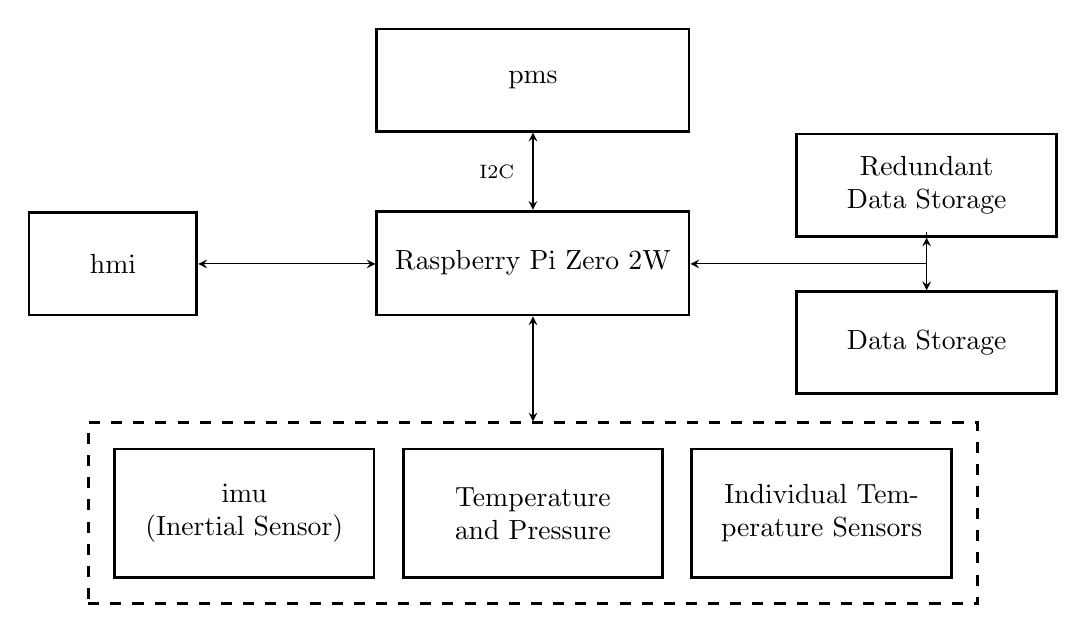
\begin{tikzpicture}
            % Paths, nodes and wires:
            \node[shape=rectangle, draw, line width=1pt, inner sep=0, minimum width=3.965cm, minimum height=1.319cm] at (9.667, 3.344){} node [anchor=center, align=center, text width=3.577cm, inner sep=5.5pt] at (9.667, 3.344){Raspberry Pi Zero 2W};
            \node[shape=rectangle, draw, line width=1pt, inner sep=0, minimum width=3.298cm, minimum height=1.631cm] at (6, 0.167){} node [anchor=center, align=center, text width=2.91cm, inner sep=5.5pt] at (6, 0.167){\acrshort{imu}\\(Inertial Sensor)};
            \node[shape=rectangle, draw, line width=1pt, inner sep=0, minimum width=3.298cm, minimum height=1.298cm] at (14.667, 4.333){} node [anchor=center, align=center, text width=2.91cm, inner sep=5.5pt] at (14.667, 4.333){Redundant Data Storage};
            \node[shape=rectangle, draw, line width=1pt, inner sep=0, minimum width=2.131cm, minimum height=1.298cm] at (4.333, 3.333){} node [anchor=center, align=center, text width=1.743cm, inner sep=5.5pt] at (4.333, 3.333){\acrshort{hmi}};
            \node[shape=rectangle, draw, line width=1pt, inner sep=0, minimum width=3.298cm, minimum height=1.631cm] at (9.667, 0.167){} node [anchor=center, align=center, text width=2.91cm, inner sep=5.5pt] at (9.667, 0.167){Temperature and Pressure};
            \node[shape=rectangle, draw, line width=1pt, inner sep=0, minimum width=3.298cm, minimum height=1.631cm] at (13.333, 0.167){} node [anchor=center, align=center, text width=2.91cm, inner sep=5.5pt] at (13.333, 0.167){Individual Temperature Sensors};
            \node[shape=rectangle, draw, line width=1pt, dash pattern={on 4pt off 4pt}, inner sep=0, minimum width=11.298cm, minimum height=2.298cm] at (9.667, 0.167){};
            \node[shape=rectangle, draw, line width=1pt, inner sep=0, minimum width=3.298cm, minimum height=1.298cm] at (14.667, 2.333){} node [anchor=center, align=center, text width=2.91cm, inner sep=5.5pt] at (14.667, 2.333){Data Storage};
            \node[shape=rectangle, draw, line width=1pt, inner sep=0, minimum width=3.965cm, minimum height=1.298cm] at (9.667, 5.667){} node [anchor=center, align=center, text width=3.577cm, inner sep=5.5pt] at (9.667, 5.667){\acrshort{pms}};
            \node[shape=rectangle, inner sep=0, minimum width=0.917cm, minimum height=0.667cm] at (9.208, 4.5){} node [anchor=center, align=center, text width=0.564cm, inner sep=5pt] at (9.208, 4.5){\scriptsize I2C};
            \draw[stealth-stealth] (7.667, 3.333) -- (5.417, 3.333);
            \draw[stealth-stealth] (9.667, 4.021) -- (9.667, 5);
            \draw[stealth-stealth] (9.667, 2.667) -- (9.667, 1.333);
            \draw[stealth-] (11.667, 3.333) -- (14.667, 3.333);
            \draw[stealth-stealth] (14.667, 3.667) -| (14.667, 3);
          \end{tikzpicture}
          \caption{Diagrama de subsistema ”On-board Computer”}
          \label{fig:sistema_obc}
        \end{figure}

      \item \textbf{Human-Machine Interface \acrshort{hmi}:} Existen dos formas principales de interactuar con
        el CubeSat. La primera es mediante llaves de hardware que se conectan físicamente al
        de interacción es a través de una interfaz web mediante protocolo HTTP, accesible mediante una
        red local generada por la \acrshort{obc}. En la Figura \ref{fig:hmi-arq} se puede ver la arquitectura
        de la página antes mencionada.

        \begin{figure}[H]
          \centering
          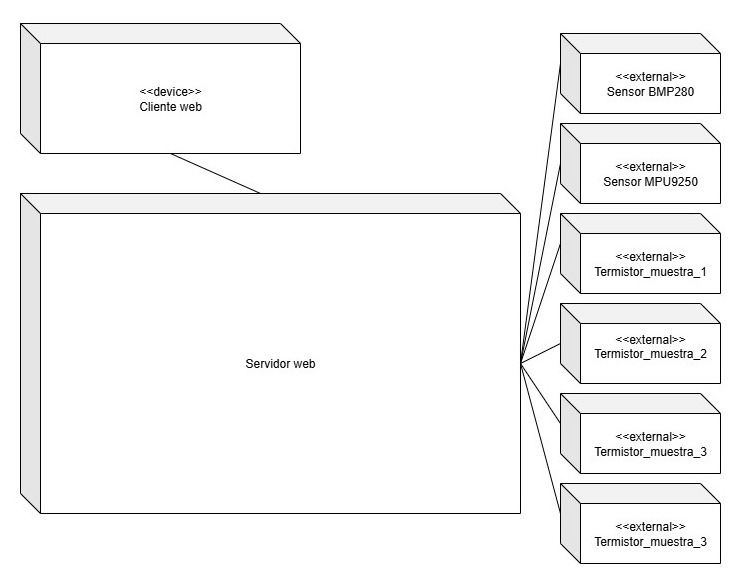
\includegraphics[width=0.6\textwidth]{image/hmi/arquitectura.jpeg}
          \caption{Vista arquitectónica despliegue}
          \label{fig:hmi-arq}
        \end{figure}

        Adicionalmente, y reservadas exclusivamente para situaciones de emergencia, estarán
        habilitadas la conexión SSH (a través de la misma red local) y la conexión UART
        mediante un puerto físico. Esta ultima constituye la única va de comunicación que
        permanece activa durante todo el ciclo operativo del CubeSat.

        Desde la interfaz web, el usuario puede consultar variables criticas del sistema (temperatura, voltajes,
        corrientes, estado de sensores, entre otros), así como habilitar o
        deshabilitar subsistemas específicos, incluyendo rieles de alimentación y módulos funcionales.

        Se pueden observar imagenes del prototípo de la interfaz web en el Anexo \ref{anexo:webpage}

        Ademas de su rol operativo, la interfaz esta diseñada también como una herramienta
        para el análisis post-misión. Una vez concluido el vuelo, permite la visualización, procesamiento
        y descarga de los archivos de datos registrados. Dicho procesamiento se realiza
        directamente en el cliente web, lo que reduce la carga sobre el sistema embarcado y
        permite un análisis dinámico sin necesidad de infraestructura adicional.

      \item \textbf{Data Storage:} La arquitectura de almacenamiento esta compuesta por dos tarjetas
        microSD de 16 GB: una como unidad principal, que aloja el sistema operativo y los
        datos primarios, y otra como unidad de respaldo, conectada mediante la interfaz SPI
        auxiliar. Ambas se encuentran configuradas en un esquema de RAID 1 por software,
        lo cual permite la replicación sincrónica de datos.

        En caso de fallos en la unidad principal
        como corrupción lógica o daño físico, un conjunto de scripts de supervisión ejecuta
        la des-conexión de la unidad afectada y procede a montar automáticamente el volumen
        redundante, asegurando as la continuidad operativa de la misión. Este mecanismo de
        conmutación automática simula un entorno de dual boot resiliente, adecuado para
        contextos de riesgo.

      \item \textbf{Environmental Sensors:} esta compuesto por los sensores encargados de medir los
        parámetros físico-ambientales durante el vuelo del CubeSat. Su función es proporcionar
        datos confiables y continuos que permitan cumplir con los objetivos establecidos en la
        misión principal, y sirvan de base contextual para interpretar los resultados de la misión
        secundaria.

        Este subsistema incluye los siguientes componentes:

        \acrfull{imu} MPU9250: permite registrar la aceleración en los
        tres ejes, as como los ángulos de orientación (roll, pitch y yaw) mediante acelerómetros,
        giroscopios y magnetómetros. Estos datos son fundamentales para la identificación de fases
        del vuelo.

        Sensor de presión y temperatura BMP280: Encargado de tomar los datos de temperatura y presión
        atmosféricas. Siendo esta última clave en la determinación de la altura del CubeSat.

      \item \textbf{Thermal Regulation Unit (\acrshort{tru}):} tiene como objetivo controlar activamente la
        temperatura de distintas muestras biológicas durante el vuelo del CubeSat, en el contexto de la
        misión secundaria. Este sistema sirve para generar condiciones térmicas
        especificas en los compartimientos que contienen los microorganismos.
        El sistema esta compuesto por los siguientes elementos principales:

      \begin{itemize}
        \item Celdas Peltier: dispositivos termoeléctricos capaces de generar un gradiente de
          temperatura al aplicarles una diferencia de potencial. Su funcionamiento permite
          tanto calentar como enfriar las muestras, dependiendo de la polaridad y nivel de
          corriente aplicada. Se utilizaran tres celdas Peltier para mantener muestras en
          temperaturas distintas.

        \item Sensores de temperatura individuales: dispuestos en cada modulo térmico, permiten medir la
          temperatura en contacto directo con las muestras, proporcionando
            una retroalimentación precisa al sistema de control.
      \end{itemize}

      El control de las celdas Peltier y la lectura de los sensores estará a cargo del \acrshort{obc}, que
      ajustara dinámicamente la potencia suministrada a cada celda a través del \acrshort{pms}.

      \item \textbf{Payload Unit:}
      subsistema pasivo que constituye el elemento central de la misión secundaria. Contiene las muestras biológicas 
      sometidas a condiciones controladas e interactúa con el \acrshort{tru}, el cual se encarga de su monitoreo y
      regulación.


    \end{itemize}

  \subsection{Herramientas de Calculo Empleadas}
    Para el desarrollo, simulación y verificación de cada uno de los subsistemas involucrados,
    se emplearan herramientas de calculo y software específicos que permitirán modelar los componentes
    y sus comportamientos, estimar el consumo de recursos, organizar la adquisición y
    el procesamiento de datos, y validar el diseño general del sistema antes de su implementación
    física.

    \begin{itemize}
      \item ANSYS Discovery (FEM)
      \item ANSYS Mechanical (FEM)
      \item Onshape (CAD)
      \item KiCad (CAD)
    \end{itemize}

  \subsection{Estructura}
    Para la estructura, tomamos inspiración de un modelo diseñado por EnduroSat \cite{endurosat}. El
    modelo esta caracterizado por el uso de estructuras fabricadas con laminas de aluminio
    plegadas, lo que le permite aprovechar al máximo el volumen del CubeSat, solo perdiendo
    dos veces el ancho de la lamina utilizada por cada eje.

    \begin{figure}[H]
      \centering
      \includegraphics[width=0.6\textwidth]{image/structure/render.png}
      \caption{Renderizado de la estructura propuesta}
      \label{fig:render}
    \end{figure}

    \subsubsection{Descripción General}

      \begin{wrapfigure}{L}{0.4\textwidth}
        \centering
        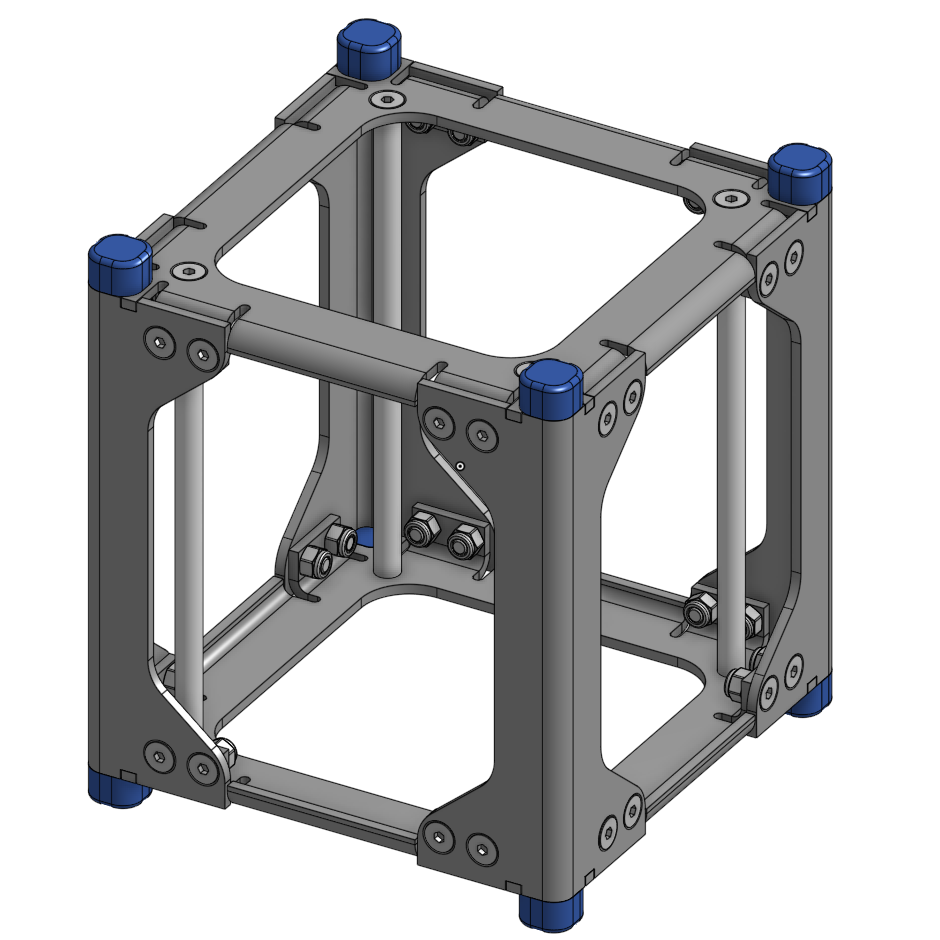
\includegraphics[width=0.4\textwidth]{image/structure/partes.png}
        \caption{Vista trimétrica}
        \label{fig:trimetrica}
      \end{wrapfigure}
      Como se mencionó previamente, la estructura del CubeSat fue diseñada a partir de láminas de aluminio
      de 2mm de espesor plegadas, para maximizar el volumen interno disponible. Esta configuración permite
      lograr una estructura rígida, de fabricación sencilla, y con un bajo peso de fabricación, gracias a
      la gran cantidad de puntos de fijación distribuidos a lo largo de la estructura.

      La estructura principal del CubeSat está compuesta por dos tapas, ubicadas en las caras +Z y -Z
      (lids), unidas entre sí mediante cuatro esquineros (corners). Todas las piezas se fijan utilizando
      tornillos M3 y tuercas autofrenantes. Los orificios de fijación están avellanados, evitando cualquier
      protrusión externa.

      La estructura del CubeSat, consta de 2 tapas, ubicadas en las caras +Z y -Z (lids), unidas a través
      de 4 esquineros (corners). La fijación de cada una de estas partes se realiza mediante tornillos y
      tuercas autofrenantes M3. Todos los agujeros llevan un corte exterior avellanado, logrando que el
      CubeSat no tenga protuberancias.

      \begin{wrapfigure}{R}{0.4\textwidth}
        \centering
        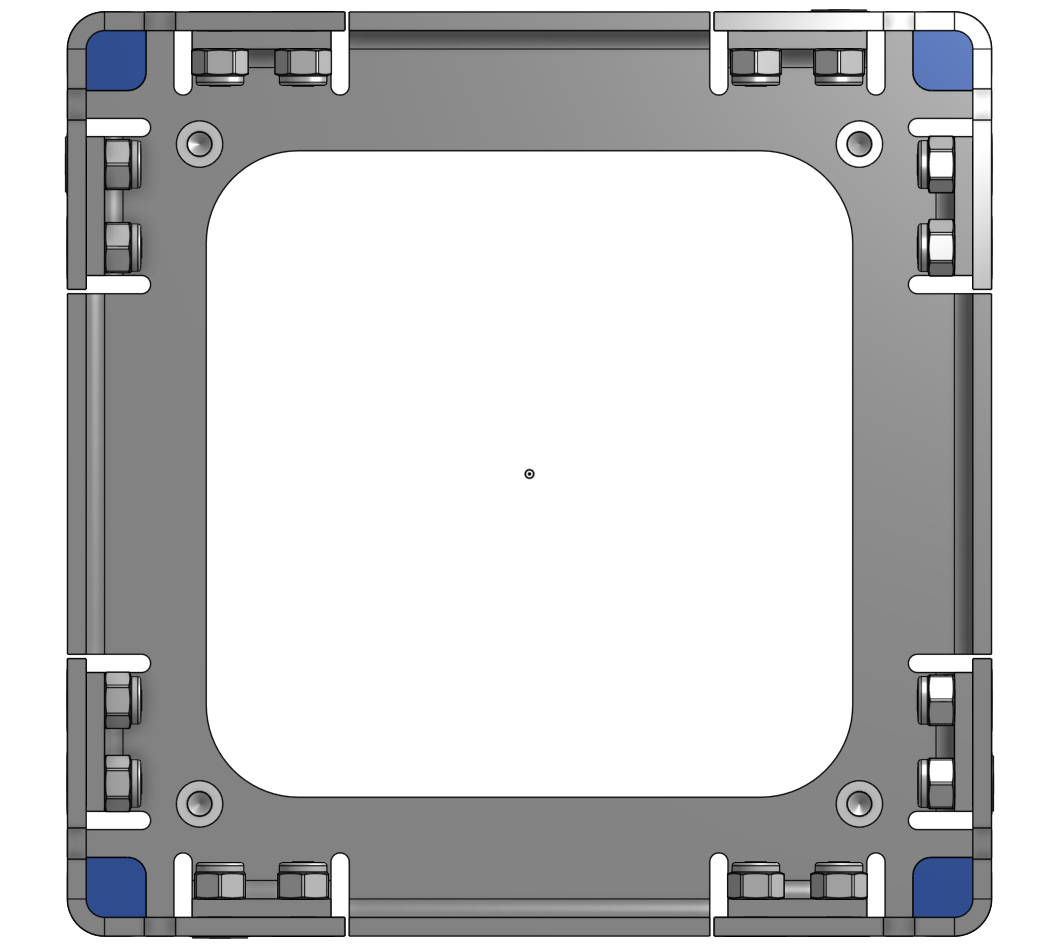
\includegraphics[width=0.4\textwidth]{image/structure/superior.png}
        \caption{Vista superior, sin tapa}
        \label{fig:superior}
      \end{wrapfigure}
      El CubeSat cuenta, además, con ocho puntos de apoyo ubicados en las caras +Y y -Y (sides),
      fabricados mediante impresión 3D por Modelado por Deposición Fundida (FDM) en polipropileno, un
      material que se seleccionó por su baja densidad, lo cual reduce la masa total del sistema, y por
      su buena capacidad de sellado y excelente adherencia entre capas, permitiendo que la resistencia
      interna del CubeSat sea hermética.

      Para el montaje de la electrónica, se diseñó una estructura interna compuesta por 3 separadores,
      los cuales fijan los módulos en los ejes X e Y, no obstante, no hay fijación en el eje Z para
      permitir el movimiento de los diferentes componentes, lo que permite aprovechar y ocupar todo el
      volumen del CubeSat.

      Los diferentes separadores se colocan de forma segura en sus correspondientes espacios en la
      estructura, y se imprimen por separado utilizando la técnica de impresión 3D (FDM) en polipropileno,
      que tiene muy buenas propiedades de adherencia entre capas, permitiendo (en caso de ser necesario)
      crear volúmenes que sean herméticos.
    \subsubsection{Proceso de Integración}

      El armado del CubeSat, comienza con la colocación de la tapa inferior (plano -Z) sobre
      el banco de armado, con los pliegues hacia arriba. A estos pliegues, se le colocan las cuatro
      esquinas, fijándolas con los tornillos y tuercas auto bloqueantes. Una vez colocados las cuatro
      esquinas, se puede proceder a colocar las varillas en la cara interna de la tapa inferior (plano
      -Z), utilizando los tornillos correspondientes.

      \begin{figure}[H]
        \begin{minipage}{0.49\textwidth}
          \centering
          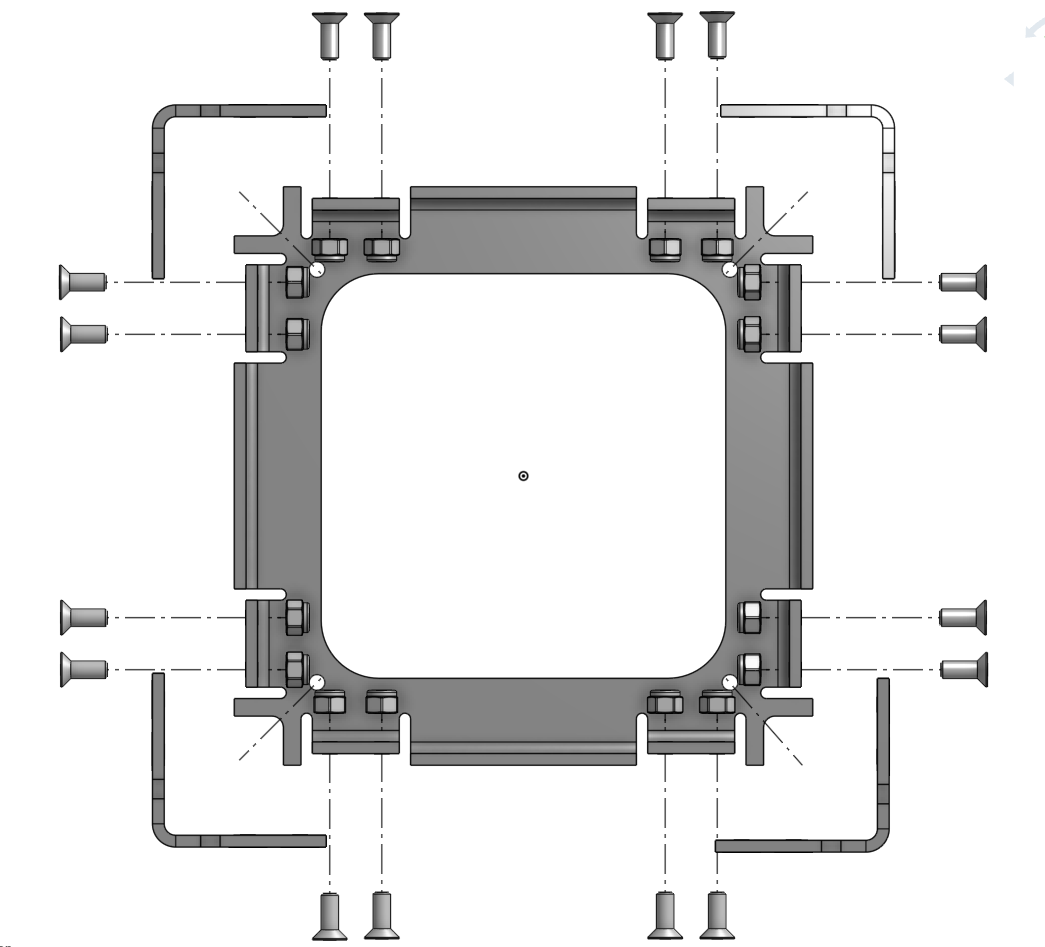
\includegraphics[width=0.9\textwidth]{image/structure/integracion1.png}
          \caption{Integración paso 1}
          \label{fig:integracion1}
        \end{minipage}
        \begin{minipage}{0.49\textwidth}
          \centering
          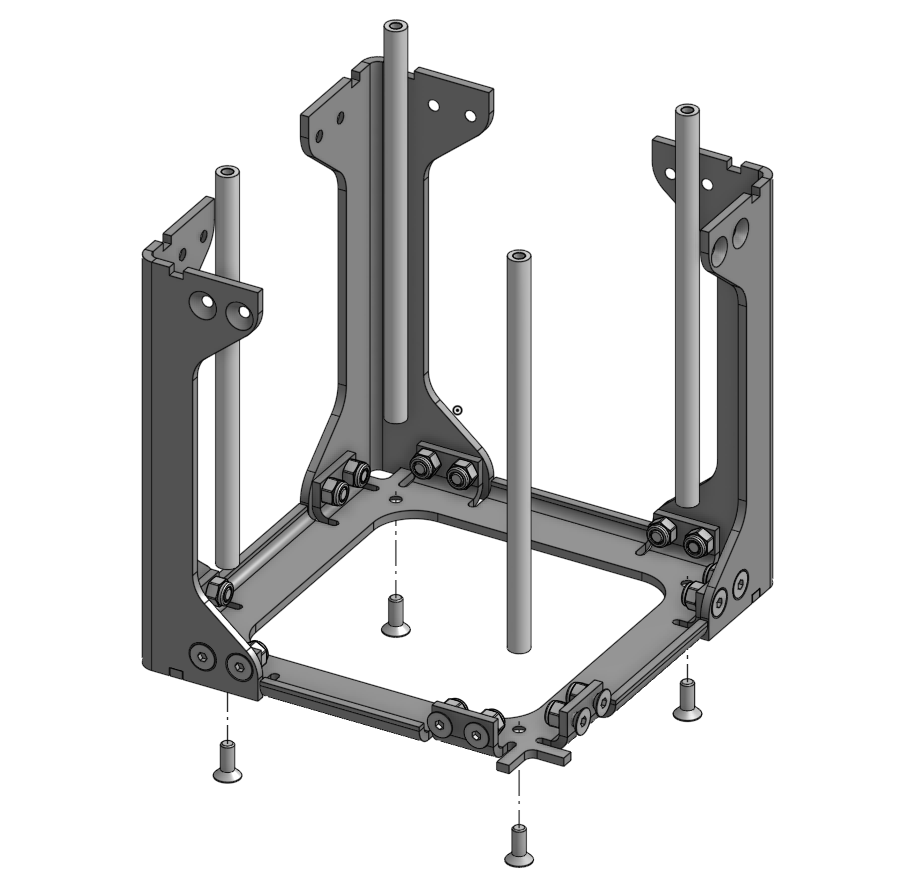
\includegraphics[width=0.9\textwidth]{image/structure/integracion2.png}
          \caption{Integración paso 2}
          \label{fig:integracion2}
        \end{minipage}
      \end{figure}

      Después de haber colocado las varillas, se puede
      proceder a colocar los diferentes subsistemas uno por uno, conectándolos entre si. Luego
      se coloca la tapa superior (plano +Z), se fijan las varillas con los tornillos, y utilizando la
      herramienta de ajuste diseñada para acceder a las tuercas superiores, se colocan los tornillos
      con las tuercas auto bloqueantes respetando el orden De esquina al centro.

      \begin{figure}[H]
        \begin{minipage}{0.49\textwidth}
          \centering
          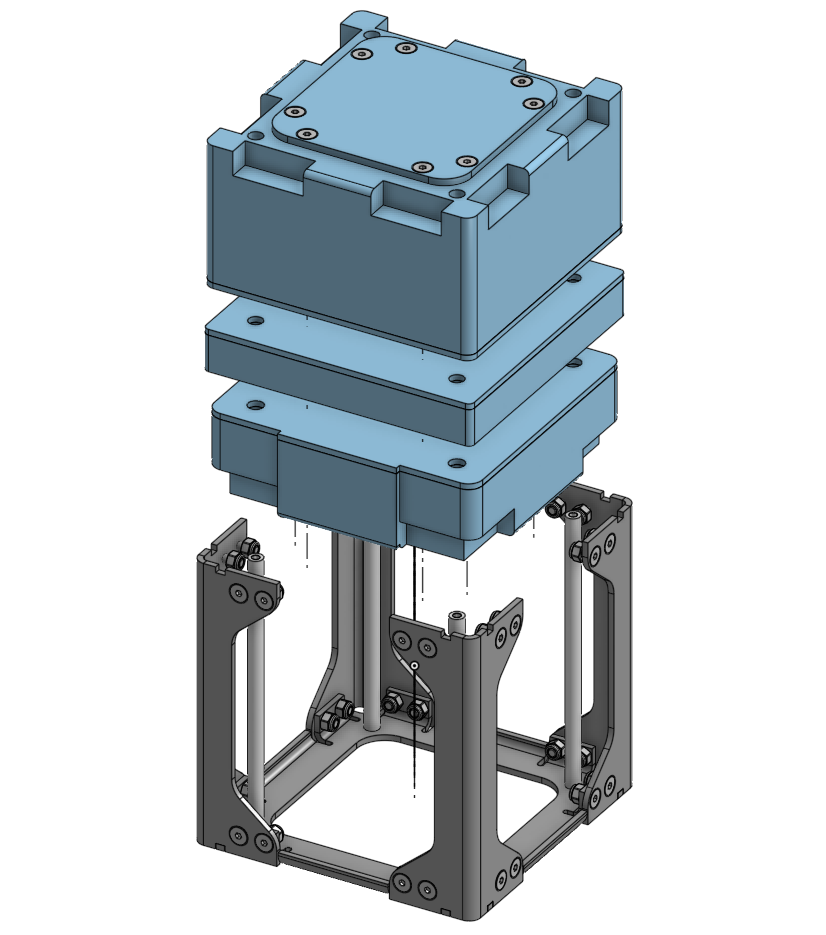
\includegraphics[width=0.9\textwidth]{image/structure/integracion3.png}
          \caption{Integración paso 3}
          \label{fig:integracion3}
        \end{minipage}
        \begin{minipage}{0.49\textwidth}
          \centering
          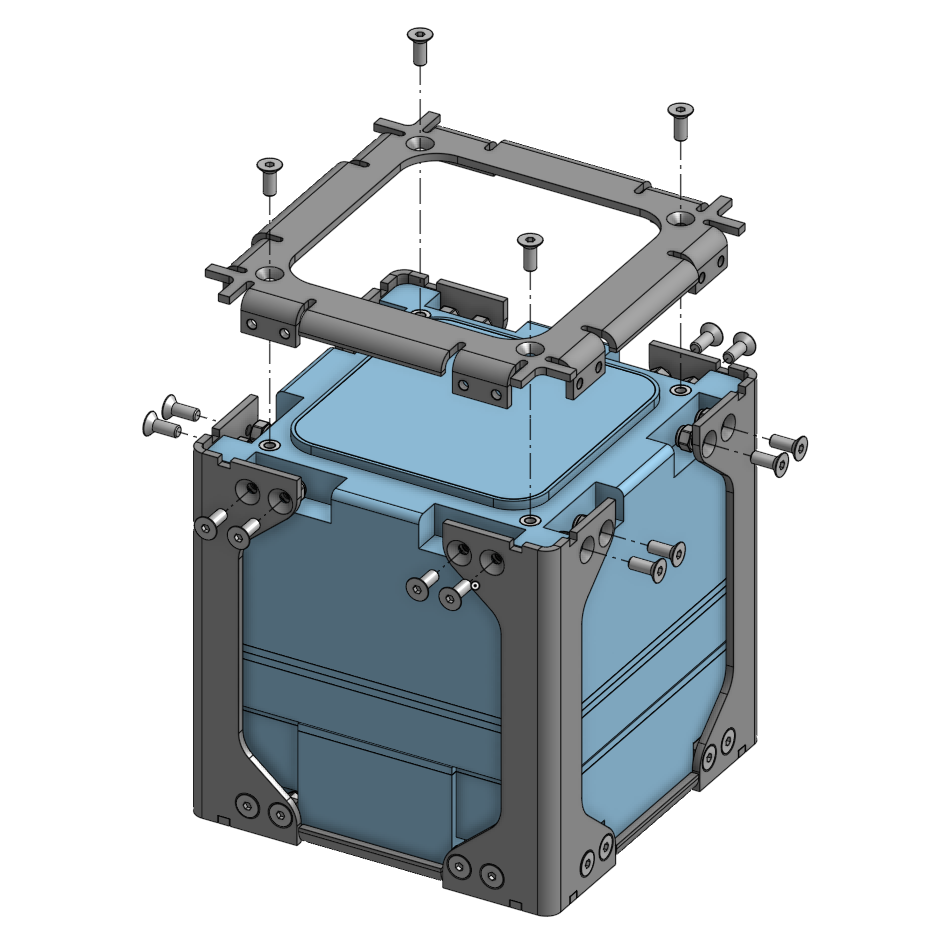
\includegraphics[width=0.9\textwidth]{image/structure/integracion4.png}
          \caption{Integración paso 4}
          \label{fig:integracion4}
        \end{minipage}
      \end{figure}

      Finalmente, se colocan los rieles a presión, para asegurar una sujeción firme
      estos deben ser enfriados previamente.
      \begin{figure}[H]
        \centering
        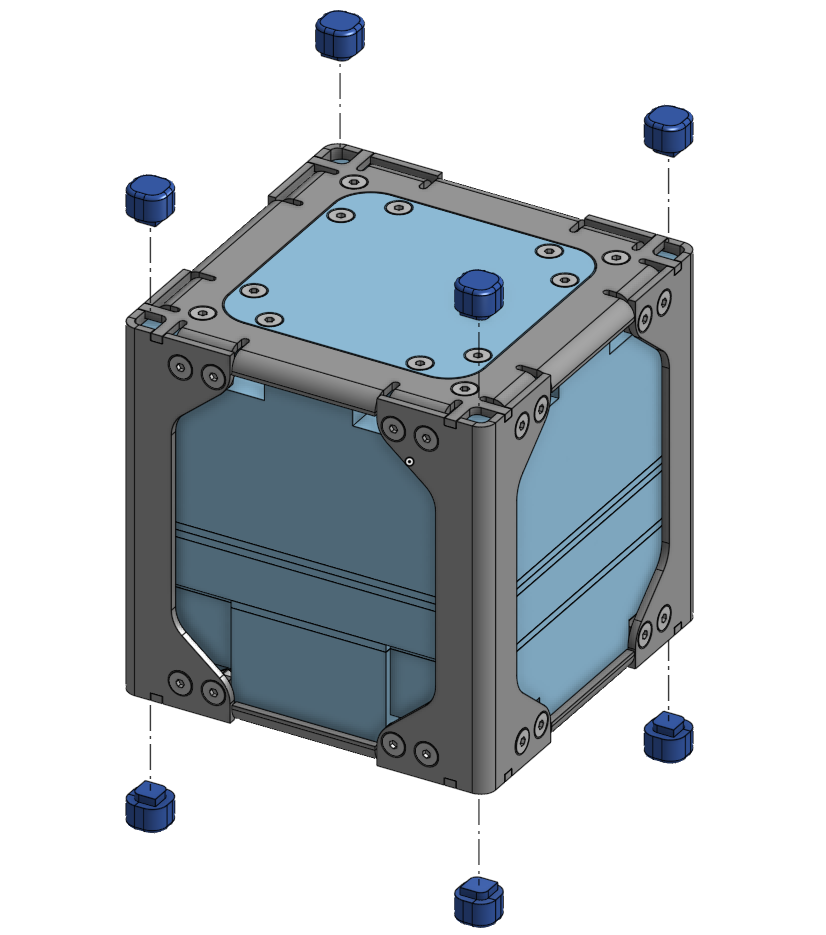
\includegraphics[width=0.4\textwidth]{image/structure/integracion5.png}
        \caption{Integración paso 5}
        \label{fig:integracion5}
      \end{figure}

    \subsubsection{Fabricación}

      La fabricación del CubeSat es relativamente simple, ya que solamente se requiere una
      plancha de aluminio como materia prima para obtener el esqueleto básico del mismo. La
      plancha de aluminio requiere ser cortada previo al plegado, ya que estos cortes implementan
      geometrías que no solo facilitan los pliegues, si no que en algunos casos los hacen posibles,
      agregando puntos de alivio. Ademas de los cortes, es necesario hacer las perforaciones necesarias
      y también los avellanados, ya que se puede dificultar hacerlos después del plegado
      debido a la complejidad de la fijación.
      \begin{figure}[H]
        \begin{minipage}{0.5\textwidth}
          \centering
          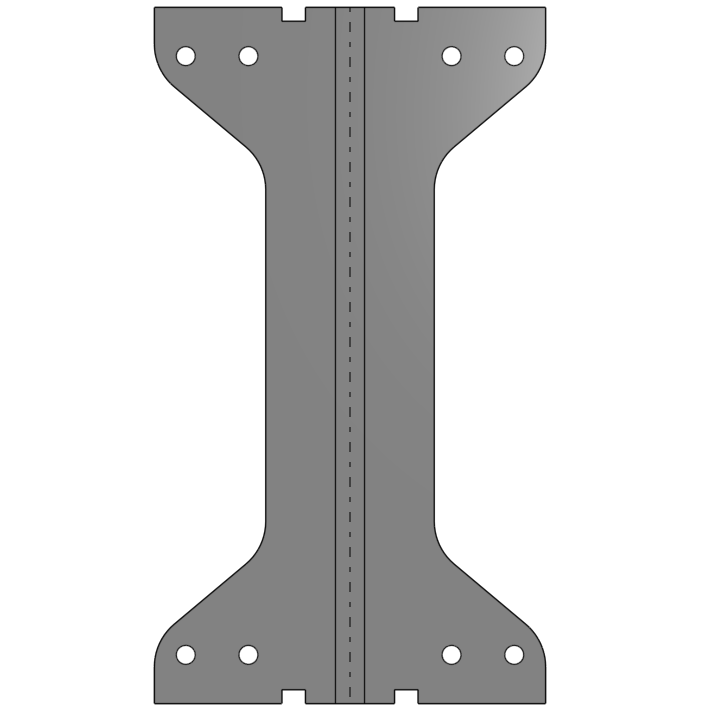
\includegraphics[width=50mm]{image/structure/cornerFlat.png}
          \caption{Corner previo al plegado}
          \label{fig:cornerfp}
        \end{minipage}
        \begin{minipage}{0.5\textwidth}
          \centering
          
\includegraphics[width=50mm]{image/structure/lidFlat.png}
          \caption{Lid previo al plegado}
          \label{fig:lidfp}
        \end{minipage}
      \end{figure}
      Los cortes de las planchas de aluminio se van a realizar utilizando una CNC, y los pliegues
      con una plegadora de chapa.
      Las varillas serán cortadas, frenteadas, perforadas y roscadas (interna) en un torno.

    \subsubsection{Colocación de Muestras}

      La estructura del CubeSat permitirá que las muestras se puedan colocar después de
      finalizar el ensamblaje de la estructura. Esto se hace posible gracias a las aberturas de las
      tapas, de las cuales la del plano +Z, va a ser para acceder a una tapa en la carcasa que aloje
      el subsistema de carga útil, y por donde se carguen las muestras a analizar. Esta tapa va a
      ser fijada con la tornillería correspondiente

      \begin{figure}[H]
        \centering
        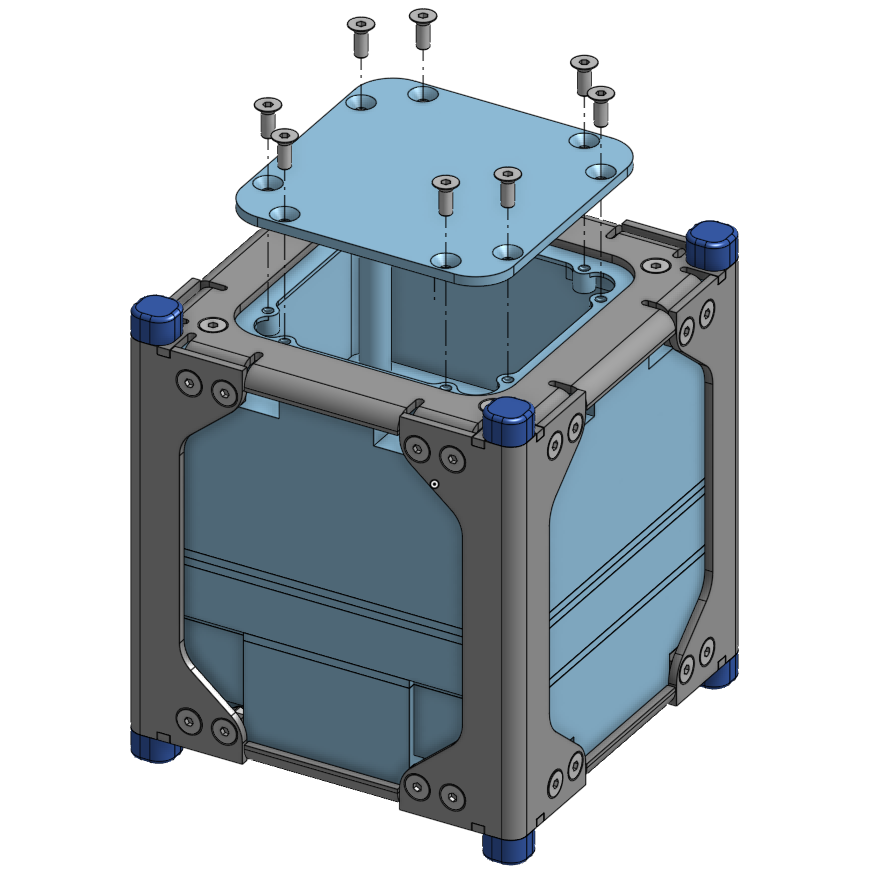
\includegraphics[width=0.4\textwidth]{image/structure/muestras.png}
        \caption{Colocacion de muestras}
        \label{fig:structure-muestra}
      \end{figure}

  \subsection{Criterios de Margenes}
    Para en análisis de presupuestos preliminares establecimos los margenes considerando las
    condiciones mas desfavorables

    \subsubsection{Presupuesto Preliminar de Masa}
      El presupuesto de masa se calcula considerando que la estructura y las baterías tienen prioridad para ser
      integradas. El sobrante (por el momento) será utilizado para los componentes internos de cada subsistema.
      \begin{table}[H]
        \centering
        \begin{tabular}{|c|c|c|c|}
          \hline
          \textbf{Elemento} & \textbf{Cantidad}                 & \textbf{Peso simple}  & \textbf{Subtotal} \\ \hline
          Lids              & 2x $10.385 \cdot 10^{-6} \, m^3$  & $2698.4 \, kg/m^3$    & $56.05 \, g$ \\ \hline
          Corners           & 4x $6.699 \cdot 10^{-6} \, m^3$   & $2698.4 \, kg/m^3$    & $72.312 \, g$ \\ \hline
          Tornillos M3      & 40                                & $0.5 \, g/u$          & $20 \, g$ \\ \hline
          Tuercas M3        & 32                                & $0.5 \, g/u$          & $16 \, g$ \\ \hline
          Baterias LiPo     & 6                                 & $50 \, g/u$           & $300 \, g$ \\ \hline
          Raspberry Pi Zero & 1                                 & $12.1 \,g/u$          & $12.1 \, g$ \\ \hline
          Celdas Peltier    & 3                                 & $24 \, g/u$           & $72 \, g$ \\ \hline
          Carcasas Subsust. & -                                 & $0,92 \, g/cm^3$      & $150 \, g$ \\ \hline
          \textbf{Total}    & -                                 & -                     & $698.46 \, g$ \\ \hline
        \end{tabular}
        \caption{Presupuesto de Pesos.}
      \end{table}

      Consideramos que con el margen de aproximadamente $300 \, g$ sobrantes, los componentes de cada subsistema
      (placas, integrados, módulos, cables, soldaduras, etc.) el CubeSat se mantendrá dentro del régimen de $1 \, Kg \pm
      20 \, g$ adaptando su posterior diseño a estas condiciones. En caso de ser necesario, se agregaran pesos
      muertos para llegar al régimen.

    \subsubsection{Presupuesto Preliminar de Potencia}
      El presupuesto de potencia se calculo considerando el caso mas desfavorable en cada uno
      de los componentes.

      \begin{table}[H]
      \centering
      \resizebox{\textwidth}{!}{
      \begin{tabular}{|l|c|c|c|c|c|c|}
      \hline
      \textbf{Componente} & \textbf{Cant.} & \textbf{Tensión [V]} & \textbf{Corriente [A]} & \textbf{Potencia [W]} & \textbf{Subtotal [W]} & \textbf{@ 7.4V[A]} \\
      \hline
      Raspberry Pi Zero 2 W & 1 & 5.0  & 260 m & 260 m & 1.3 & 175.67 m   \\
      Atmega328p            & 1 & 5.0  & 5.2 m & 26 m & 26 m  & 3.5 m   \\
      Sensor BMP280         & 1 & 3.3  & 0.7 m & 2.3 m & 2.3 m & 0.310 m \\
      Sensor MPU9250        & 1 & 3.3  & 3.9 m & 12.9 m & 12.9 m & 1.74 m\\
      TB6612FNG             & 2 &  -   &   -   & 1 * canal & 3 & 405.54 m\\
      Celdas Peltier 4x4 cm & 3 & 12.0 & 833 m & 10.00  & 30.00  & 4.05   \\
      \hline
      \textbf{Total}        & – & –   & –      & –      & \textbf{34.34} & \textbf{4.63} \\
      \hline
      \end{tabular}
      }
      \caption{Consumo de corriente y potencia de los componentes en el caso más desfavorable.}
      \label{tab:consumo_componentes}
      \end{table}

      Para la mision elegimos tener 6 celdas 18650 de 3.7 V cada una con una capacidad de 3200 mAh. Se dispondran de
      manera que habra 2 conexiones en serie y 3 conexiones en paralelo, teniendo en total 7.4 V y 9600 mAh. Esto nos
      dará un tiempo de autonomia de 124 minutos. Esto es considerando casos mas desfavorables. Para el futuro, se
      buscara hacer ensayos reales del consumo de cada componente y se buscara que cada uno de ellos sea el menor posible.
      Para determinar la potencia de los sensores se ha considerado sus respectivos datasheet \cite{datasheet-mpu9250} \cite{datasheet-bpm280}.

    \subsubsection{Presupuesto Preliminar de Datos}
      Durante el vuelo se generaran y almacenaran diversos tipos de datos relacionados tanto
      con la misión primaria como con la misión secundaria. A continuación se detalla el presupuesto preliminar de almacenamiento de datos considerando un periodo de recolección de 4
      horas.
      Cada muestra registrada incluye el instante temporal y el valor medido del parámetro, ocupando 4 bytes cada uno, lo que da un total de 8 bytes por muestra. Ademas, consideramos
      la mayor frecuencia de muestreo permitida por cada sensor.

      \begin{table}[H]
      \centering
      \begin{tabular}{|l|c|}
      \hline
      \textbf{Vector} & \textbf{Tamaño de muestra} \\
      \hline
      Tiempo & 4 bytes \\
      Valor  & 4 bytes \\
      \hline
      \textbf{Tamaño total} & \textbf{8 bytes} \\
      \hline
      \end{tabular}
      \caption{Tamaño total fijo por muestra de cada parámetro}
      \label{tab:tamanio_muestra}
      \end{table}

      \begin{itemize}

        \item \textbf{Variables físicas y ambientales}

        \begin{table}[H]
        \centering
        \begin{tabular}{|l|c|c|c|c|}
        \hline
        \textbf{Parámetro} & \textbf{Tipo} & \textbf{Frecuencia [Hz]} & \textbf{Muestras/4h} & \textbf{Tamaño [MB]} \\
        \hline
        Presión               & float & 157   & 2,260,800  & $\approx$ 8.63     \\
        Temperatura ambiente  & float & 157   & 2,260,800  & $\approx$ 8.63     \\
        Aceleración           & float & 4000  & 5,760,000  & $\approx$ 219.73   \\
        Ángulo de giro        & float & 8000  & 11,520,000 & $\approx$ 439.45   \\
        \hline
        \textbf{Total estimado} & -    & -     & -         & $\boldsymbol{\approx 685.07}$ \\
        \hline
        \end{tabular}
        \caption{Volumen de datos total y de cada variable físico-ambiental}
        \label{tab:volumen_datos}
        \end{table}

        \item \textbf{Control de temperatura de de las muestras celulares}

        \begin{table}[H]
        \centering
        \begin{tabular}{|l|c|c|c|c|}
        \hline
        \textbf{Parámetro} & \textbf{Tipo} & \textbf{Frecuencia [Hz]} & \textbf{Muestras/4h} & \textbf{Tamaño [MB]} \\
        \hline
        Temperatura ideal de cultivo & float & 157 & 2,260,800 & $\approx$ 8.63 \\
        Temperatura menor            & float & 157 & 2,260,800 & $\approx$ 8.63 \\
        Temperatura mayor            & float & 157 & 2,260,800 & $\approx$ 8.63 \\
        Temperatura ambiente         & float & 157 & 2,260,800 & $\approx$ 8.63 \\
        \hline
        \textbf{Total estimado}      & -     & -   & -         & $\boldsymbol{\approx 34.52}$ \\
        \hline
        \end{tabular}
        \caption{Volumen de datos de los controles de temperatura de las muestras celulares}
        \label{tab:volumen_datos_temperatura}
        \end{table}

        \item \textbf{Información gravada previamente}

        \begin{table}[H]
        \centering
        \begin{tabular}{|l|c|c|}
        \hline
        \textbf{Software} & \textbf{Versión} & \textbf{Tamaño} \\
        \hline
        S.O. Raspberry Pi OS Lite (Debian 12.0 "bookworm") & - & $\approx$ 2.1~GB \\
        Python                   & 3 & $\approx$ 27.5~\textit{MB} \\
        Dependencias python      & 1 & $\approx$ 150~\textit{MB} \\
        logrotate                & 1 & $\approx$ 100~\textit{KB} \\
        chrony                   & 1 & $\approx$ 2~\textit{MB} \\
        \hline
        \textbf{Total estimado}  & - & $\boldsymbol{\approx 2.3~GB}$ \\
        \hline
        \end{tabular}
        \caption{Consumo de almacenamiento de los componentes}
        \label{tab:almacenamiento_componentes}
        \end{table}
    
      \end{itemize}

      \begin{table}[H]
      \centering
      \begin{tabular}{|l|c|}
      \hline
      \textbf{Apartado} & \textbf{Tamaño estimado [MB]} \\
      \hline
      Variables físicas              & 685.07 \\
      Back up Variables físicas      & 685.07 \\
      Temperaturas celulares         & 34.52  \\
      Back up Temperaturas celulares & 34.52  \\
      Información grabada previamente & 2355 \\
      \hline
      \textbf{Tamaño total}          & \textbf{3794.3} \\
      \hline
      \end{tabular}
      \caption{Tamaño total estimado}
      \label{tab:tamano_total_estimado}
      \end{table}

      Teniendo en cuenta todos los datos a ser almacenados, estimamos un volumen total de
      aproximadamente 3.7 GB

\section{Secuencia de Operación}
  Para poder llevar a cabo la misión, es necesario obtener las muestras primero. Para la obtención de las muestras, se
  utilizaran las instalaciones mas cercanas a la zona de lanzamiento, para cultivar las muestras varios días antes del
  día de lanzamiento. Una vez cultivadas las muestras, el día antes o durante el mismo día del lanzamiento, se buscan
  las muestras para ser almacenadas en un lugar seguro durante toda la secuencia de lanzamiento hasta que haya que
  cargar las muestras en el CubeSat.

  Para el día del lanzamiento, se provee que que todo el evento siga la siguiente secuencia:
  \begin{itemize}
    \item \textbf{Etapa 1:} Arranque del CubeSat.\\
      Durante esta etapa, se enciende el CubeSat, y se coloca la llave de Pre Lanzamiento, la cual inicializara todos
      los subsistemas. En esta etapa, el CubeSat puede ser conectado a una fuente de alimentación externa para hacer que
      la entrada en régimen permanente para la temperatura de la bahía de muestras no consuma mucha batería por el pico inicial
      de cambio de temperatura requerido.
    \item \textbf{Etapa 2:} Validación de los sistemas.\\
      Mientras el CubeSat estabiliza la temperatura en modo Pre Lanzamiento, se abre un canal de comunicación con el
      CubeSat vía WiFi, al cual uno de los integrantes de Software y Hardware se conectaran mediante una computadora,
      para hacer la validación de todos los sensores, y verificar que estén en estados operativos. También, se
      corroboraran los voltajes y consumos reportados de las baterías, para verificar que también se encuentren en
      niveles óptimos.
    \item \textbf{Etapa 3:} Colocación de las Muestras.\\
      Una vez que la temperatura de la bahía de muestras ya esta estabilizada y asegurada, se procede a destapar la
      bahía de muestras, para la posterior colocación de las mismas. La colocación de las muestras va a generar una
      diferencia en la temperatura, por lo que es requisito estar monitoreando que la misma no varié demasiado del punto
      configurado para evitar estresar los organismos presentes en las muestras.
    \item \textbf{Etapa 4:} Preparación para el lanzamiento.\\
      Con el CubeSat en estado de Pre Lanzamiento, todos los sensores verificados, y todas las muestras cargadas, se
      procede a fijar todas las tapas, desconectar la fuente de alimentación externa, y cargar el CubeSat a la bahía de
      carga del Cohete. En este estado, el CubeSat seguirá teniendo el puerto de comunicación vía WiFi disponible, hasta
      que se retire la llave de Pre Lanzamiento o "Remove Before Flight".
    \item \textbf{Etapa 5:} Lanzamiento, apogeo y aterrizaje.\\
      Durante esta etapa, no hay telemetría que recibir, ni parámetros que monitoreos. Solo se mantienen las muestras
      terrestres en condiciones optimas, las cuales van a ser comparadas con las del CubeSat una vez sea recuperado.
    \item \textbf{Etapa 6:} Recuperación del CubeSat.\\
      Una vez recuperado el CubeSat, se colocara la llave de recuperación de datos, y se colocara la fuente de
      alimentación externa para evitar dañar las baterías y mantener las muestras estables. Con la fuente conectada, se
      procede a extraer las muestras de la bahía de muestras, para su posterior almacenaje en un medio seguro y bajo en
      estrés. Al mismo tiempo, integrantes del equipo de Software y Hardware se encargaran de realizar la descarga de
      los datos del CubeSat a una plataforma local para su posterior procesamiento.
    \item \textbf{Etapa 7:} Procesamiento de datos.\\
      Con los datos del CubeSat descargados y guardados en un lugar seguro, se puede colocar la llave de apagado del
      CubeSat y desconectar la fuente externa. Con las herramientas desarrolladas por el equipo de software, se
      realizara el procesamiento de las muestras, para buscar patrones y presentarlos en un informe.
    \item \textbf{Etapa 8:} Control de las muestras.\\
      Con el equipo requerido, se hará la comparación de las muestras de tierra, las muestras del CubeSat y las muestras
      de laboratorio, en búsqueda de fluctuaciones en la reproducción de las células, cantidad de células muertas y
      alteraciones provocadas en las mismas por sus sistemas de defensa basados en estrés.
    \item \textbf{Etapa 9:} Presentación de los datos.\\
      Los informes son presentados con conclusiones respecto a los resultados obtenidos durante el lanzamiento.
  \end{itemize}

\section{Aseguramiento de Misión}

  \subsection{Análisis de Confiabilidad}
    Para el análisis de la confiabilidad de la estructura del CubeSat, se empleo el suite de herramientas de ANSYS, en
    su versión educativa. El suite provee un extenso catalogo de herramientas de análisis y simulaciones y a su vez un
    amplio catalogo de materiales con todas sus propiedades. Para nuestro CubeSat, decidimos emplear los análisis
    modales, de vibraciones aleatorias y de estructura estática, de los cuales obtuvimos métricas como la fatiga en
    diferentes puntos de la estructura, deformaciones dadas las condiciones de prueba y factor de seguridad para
    diferentes puntos.

    Para las simulaciones fue necesario elegir un material para cada elemento separado que forma parte de la estructura.
    En el Cuadro \ref{tab:materiales_empleados} se puede ver la lista de materiales empleados y algunas de sus
    propiedades importantes.

    \begin{table}[H]
    \centering
    \small
    \begin{tabular}{|p{2.2cm}|p{2.3cm}|p{2.3cm}|p{2.5cm}|p{2cm}|p{2.5cm}|}
    \hline
    \textbf{Material} & \centering\textbf{Módulo de elasticidad} & \centering\textbf{Límite Elástico} & \centering\textbf{Límite de Rotura} & \centering\textbf{Densidad} & \centering\textbf{Usado en} \tabularnewline
    \hline
    Aleación de Aluminio & \centering $71 \cdot 10^9\,Pa$ & \centering $280 \cdot 10^6\,Pa$ & \centering $310 \cdot 10^6\,Pa$ & \centering $2770\,kg/m^3$ & Tapas y Esquinas \tabularnewline
    \hline
    Acero 4140 & \centering $212.5 \cdot 10^9\,Pa$ & \centering $652.2 \cdot 10^6\,Pa$ & \centering $1015 \cdot 10^6\,Pa$ & \centering $7850\,kg/m^3$ & Tornillería y Varillas \tabularnewline
    \hline
    Polipropileno & \centering $1461 \cdot 10^6\,Pa$ & \centering $34.6 \cdot 10^6\,Pa$ & \centering $37.62 \cdot 10^6\,Pa$ & \centering $903.4\,kg/m^3$ & Rieles de Apoyo y carcasas \tabularnewline
    \hline
    \end{tabular}
    \caption{Lista de materiales empleados.}
    \label{tab:materiales_empleados}
    \end{table}

    Debido a que aun no esta completamente definido como será la disposición interna de cada subsistema del CubeSat,
    para las simulaciones colocamos objetos que tienen las mismas dimensiones y materiales de las carcasas de los
    subsistemas, pero solidos (rellenos) y ajustados para que tengan el peso necesario para que el CubeSat llegue al
    kilogramo.

    \subsubsection{Preparación del modelo}
      \begin{wrapfigure}{r}{0.4\textwidth}
        \vspace{-0.5cm}
        \centering
        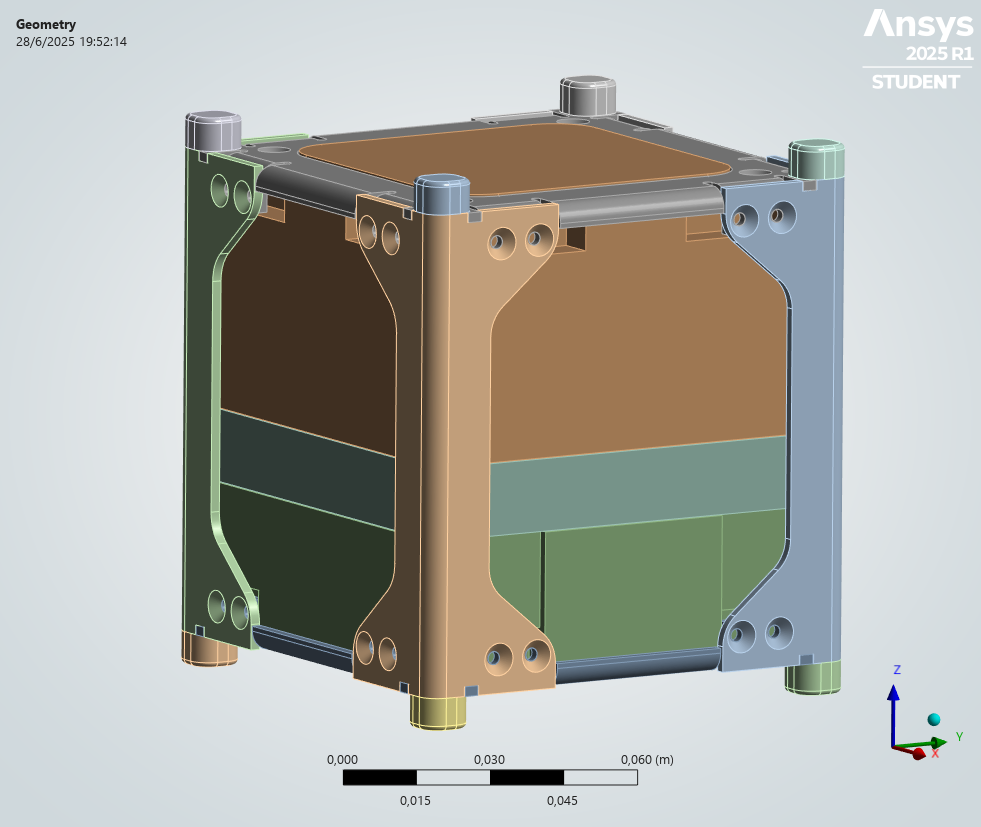
\includegraphics[width=0.4\textwidth]{image/fem/ansys_cubesat-geometry.png}
        \caption{Geometría importada}
        \label{fig:fem_geo}
      \end{wrapfigure}
      \hspace*{2em}
      El ensamblaje del CubeSat se exporta desde la plataforma de CAD online utilizada (Onshape) en formato STEP. De
      ahí, se importa la geometría a ANSYS Mechanical, el cual nos permite crear la selección y asignación de los
      materiales, fijar superficies de contacto y establecer superficies de fijación. Luego de importar la geometría,
      ANSYS Mechanical automáticamente genera la malla para su posterior uso en simulación.  Es importante mencionar que
      para las simulaciones, los tornillos y tuercas no están siendo tomados en cuenta. Esto se debe a que la
      complejidad que le agrega a la malla, y la cantidad de nodos que son necesarios para poder incluir las 32 tuercas
      y los 40 tornillos a la malla y al análisis, excede los limites de la licencia educativa por la cual estamos
      haciendo uso del software. En la figura \ref{fig:fem_mesh} se puede ver la malla generada.

      Para la correcta visualización de las imágenes presentes en esta sección serán anexadas en el mayor tamaño posible
      en el Anexo\ref{anexo:simulaciones}

      \begin{figure}[H]
        \centering
        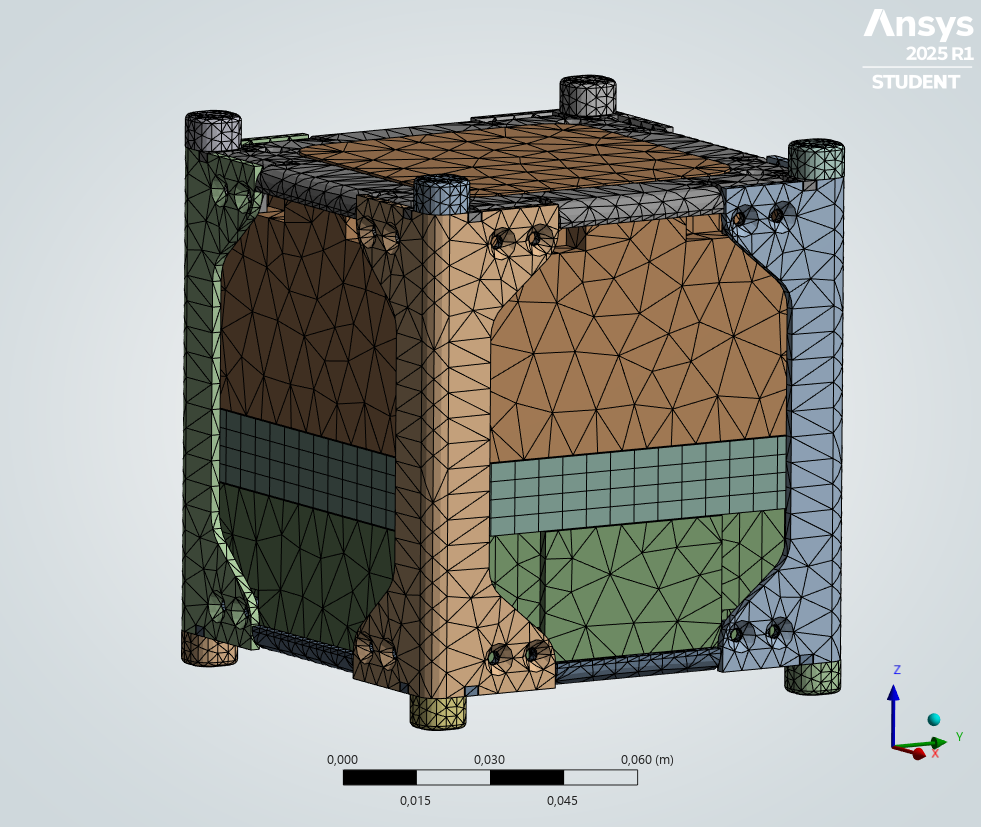
\includegraphics[width=0.7\textwidth]{image/fem/ansys_cubesat-mesh.png}
        \caption{Malla generada automáticamente por ANSYS Mechanical}
        \label{fig:fem_mesh}
      \end{figure}

    \subsubsection{Análisis Modal}

      Para poder proceder a las simulaciones de vibraciones aleatorias (workmanship) y análisis de integridad
      estructural, es necesario determinar las frecuencias modales del CubeSat. En el Cuadro \ref{tab:modos_obtenidos}
      se pueden ver las frecuencias modales encontradas desde 0Hz hasta 2200Hz.

      \begin{table}[H]
      \centering
      \begin{tabular}{|c|c|c|c|c|c|c|}
      \hline
      \textbf{Modo}       & 1           & 2           & 3           & 4         & 5           & 6          \\
      \hline
      \textbf{Frecuencia} & $536.89\,Hz$ & $541.52\,Hz$ & $908.97\,Hz$ & $1253\,Hz$ & $1616.2\,Hz$ & $1624.1\,Hz$ \\
      \hline
      \end{tabular}
      \caption{Modos obtenidos.}
      \label{tab:modos_obtenidos}
      \end{table}

    \subsubsection{Análisis de Vibraciones Aleatorias}

      En este análisis, se sometió el CubeSat a la curva $G^2/Hz$ recomendada por la competencia. Como ANSYS Mechanical
      ya tiene incorporado el mecanismo para conectar puntos por tramos rectos, la curva resultante tiene que pasar por
      los puntos especificados en el cuadro \ref{tab:accel}, generando una curva como la de la figura
      \ref{fig:graph_accel}.

      \begin{figure}[!ht]
        \centering
        \begin{minipage}{0.4\textwidth}
          \centering
          \begin{tabular}{|c|c|}
            \hline
            Frecuencia & Aceleracion G \\ \hline
            $20 \, Hz$ & $0.01 \, G^2/Hz$ \\ \hline
            $80 \, Hz$ & $0.04 \, G^2/Hz$ \\ \hline
            $500 \, Hz$ & $0.04 \, G^2/Hz$ \\ \hline
            $2000 \, Hz$ & $0.01 \, G^2/Hz$ \\ \hline
          \end{tabular}
          \captionof{table}{Puntos de aceleraciones G segun frecuencia.}
          \label{tab:accel}
        \end{minipage}
        \hspace{0.05\textwidth}
        \begin{minipage}{0.4\textwidth}
          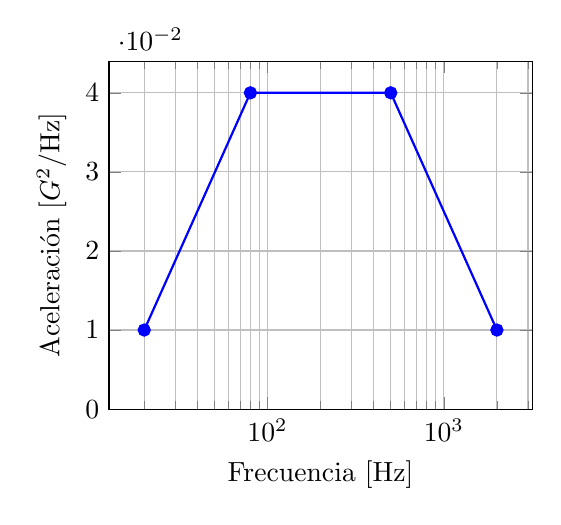
\begin{tikzpicture}
            \begin{axis}[
              xmode=log,
              xlabel={Frecuencia [Hz]},
              ylabel={Aceleración [$G^2$/Hz]},
              grid=both,
              ymin=0,
              height=6cm,
            ]
              \addplot[
                color=blue,
                mark=*,
                thick
              ] coordinates {
                (20, 0.01)
                (80, 0.04)
                (500, 0.04)
                (2000, 0.01)
              };
            \end{axis}
          \end{tikzpicture}
          \caption{Curva con los puntos interpolados de aceleración G.}
          \label{fig:graph_accel}
        \end{minipage}
      \end{figure}

      Esta curva se aplica a los tres ejes del CubeSat, lo que permite generar los análisis de estrés y tensión.

      \begin{figure}[H]
        \begin{minipage}{0.5\textwidth}
          \centering
          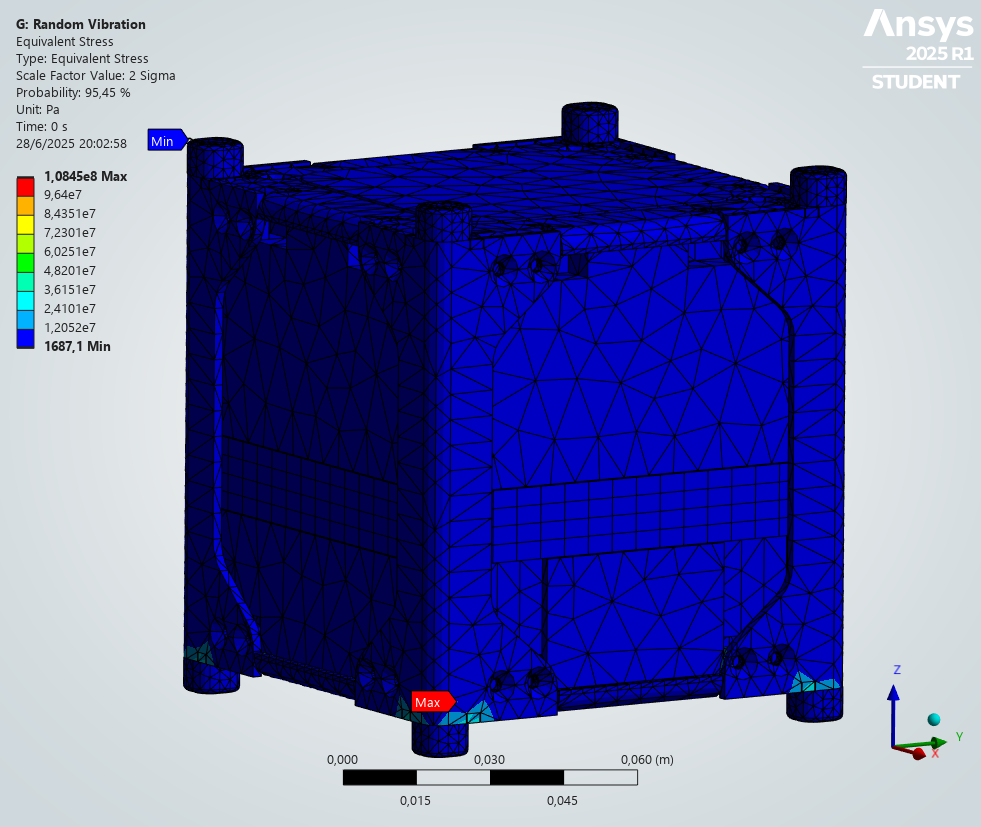
\includegraphics[width=\textwidth]{image/fem/ansys_cubesat-vibration_stress.png}
          \caption{Análisis de estrés}
          \label{fig:fem_stress}
        \end{minipage}
        \begin{minipage}{0.5\textwidth}
          \centering
          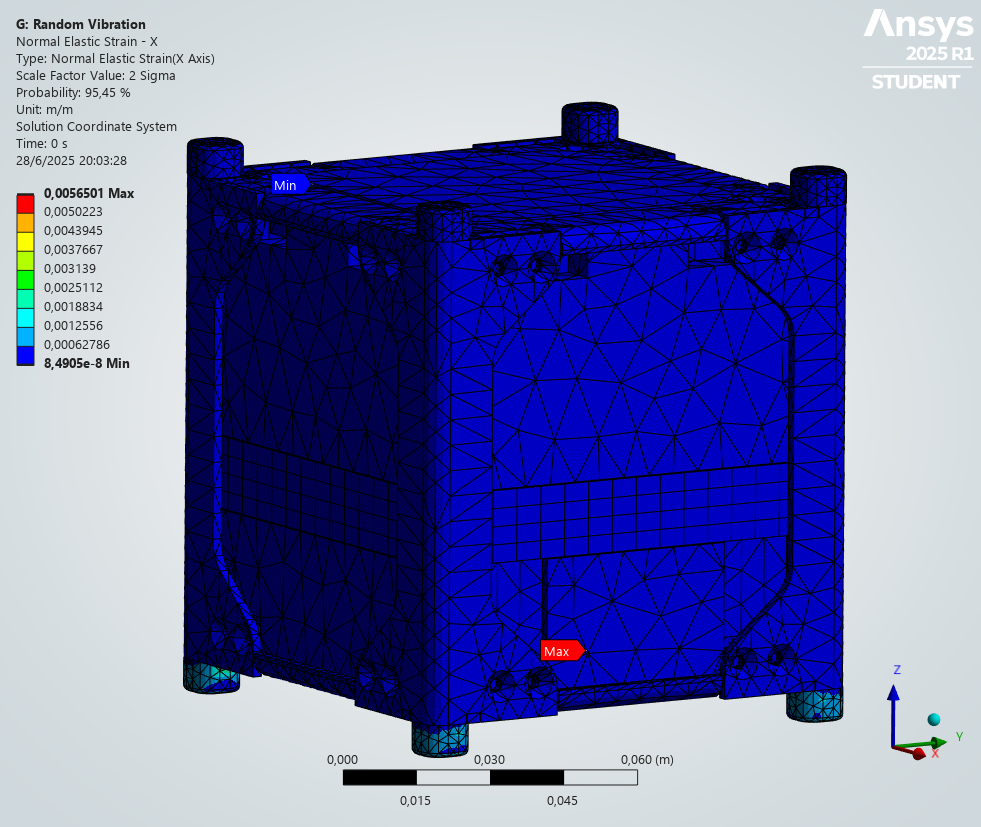
\includegraphics[width=\textwidth]{image/fem/ansys_cubesat-vibration_strain-x.png}
          \caption{Análisis de tensión en el eje x}
          \label{fig:fem_strain-x}
        \end{minipage}
      \end{figure}
      \begin{figure}[H]
        \begin{minipage}{0.5\textwidth}
          \centering
          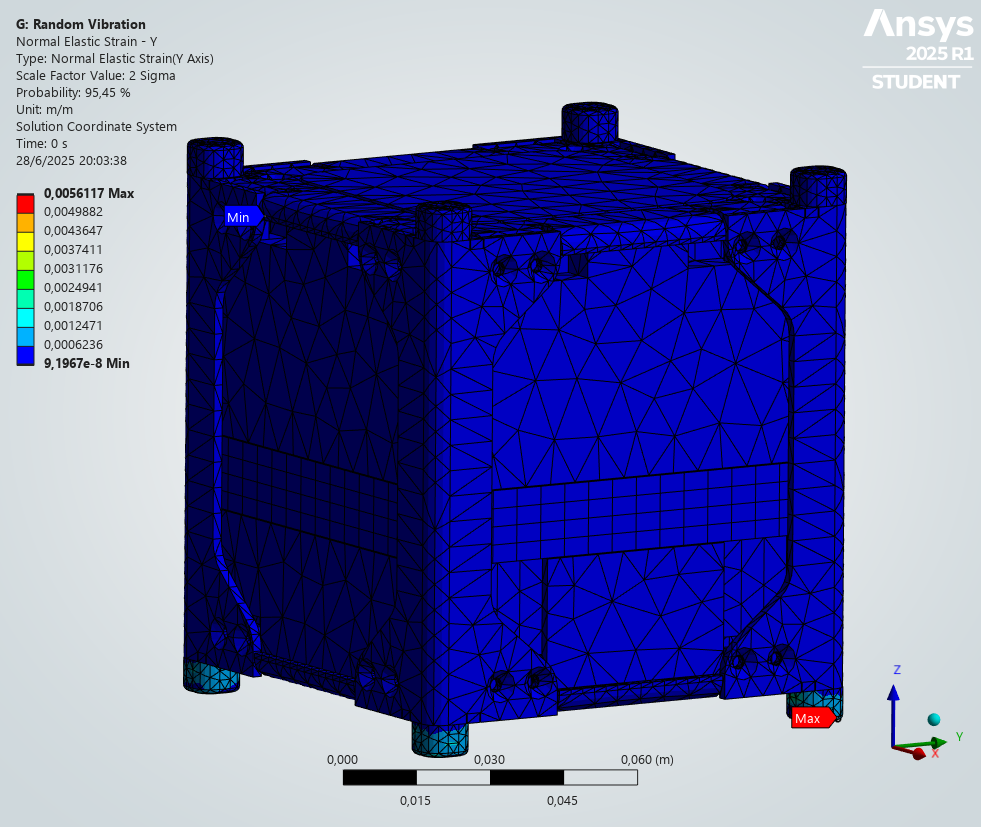
\includegraphics[width=\textwidth]{image/fem/ansys_cubesat-vibration_strain-y.png}
          \caption{Análisis de tensión en el eje Y}
          \label{fig:fem_strain-y}
        \end{minipage}
        \begin{minipage}{0.5\textwidth}
          \centering
          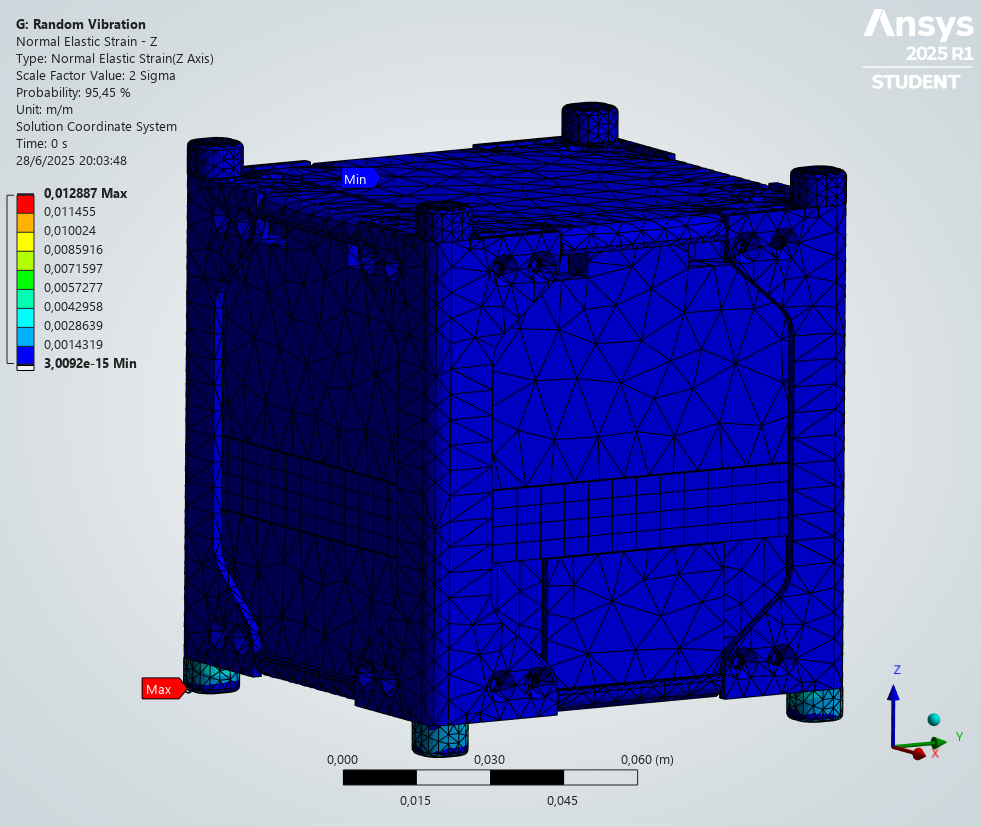
\includegraphics[width=\textwidth]{image/fem/ansys_cubesat-vibration_strain-z.png}
          \caption{Análisis de tensión en el eje Z}
          \label{fig:fem_strain-z}
        \end{minipage}
      \end{figure}

      Como se puede ver en la figura \ref{fig:fem_stress}, para el análisis de estrés equivalente, el pico máximo es de
      $108.106 \, Pa$. Analizando con mas detalle, este punto se encuentra en la superficie de contacto de la tapa
      inferior y la varilla. Debido al limite de resolución, este punto de alta presión puede ser una falla de
      simulación, pero en caso de que no lo sea, sigue estando por debajo del limite de rotura del aluminio y del acero,
      por lo que no presenta un problema.

    \subsubsection{Análisis Estático}
      \begin{wrapfigure}{R}{0.4\textwidth}
        \vspace{-0.5cm}
        \centering
        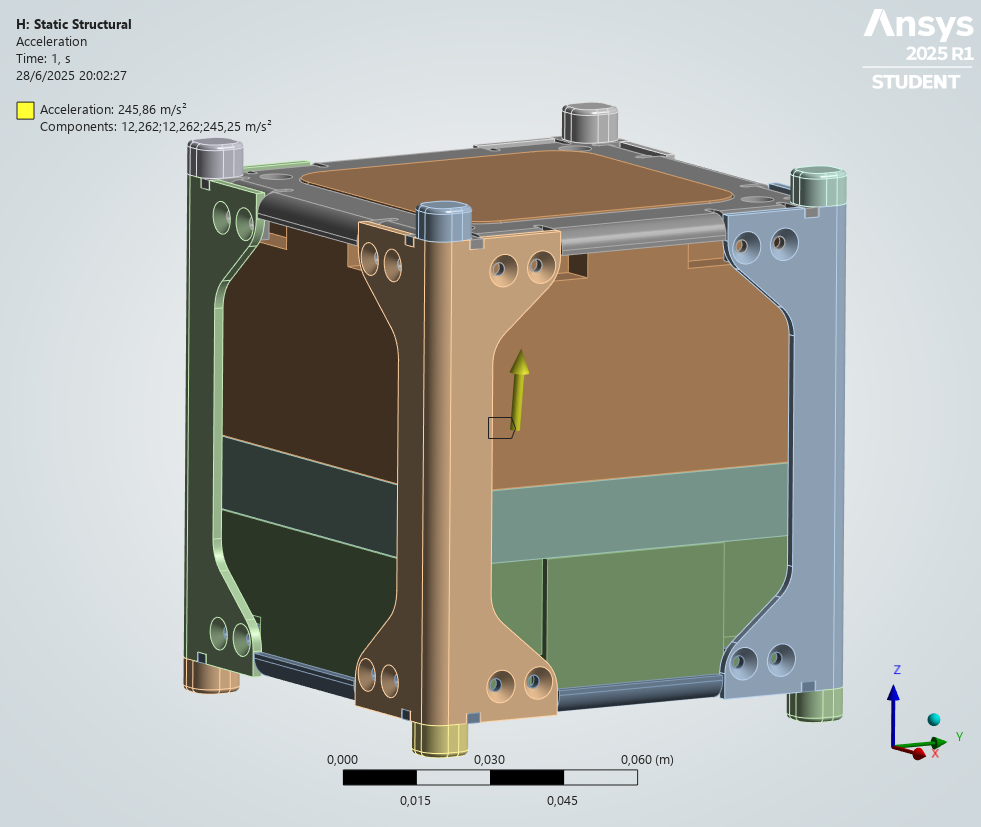
\includegraphics[width=0.33\textwidth]{image/fem/ansys_cubesat-static_acceleration.png}
        \caption{Vector de aceleración para la simulación estática.}
        \label{fig:fem_static_acc}
      \end{wrapfigure}

      Se espera que el CubeSat este sometido a una aceleraciones de hasta 20g en el sentido +z y hasta 1g en los
      sentidos x e y. Para las simulaciones, se utilizaron estos valores con un factor de 1.25x. Un detalle que cabe
      destacar, es que todas las deformaciones presentes en estas simulaciones, están amplificadas visualmente para
      facilitar la detección patrones y fallas en el diseño de la estructura, por lo tanto, es fundamental interpretar
      los resultados en función de las escalas de color y los valores numéricos de los distintos análisis, y no tomar
      como referencia la magnitud visual de las deformaciones mostradas. Aclarado esto, se muestran a continuación las
      simulaciones realizadas.

      \begin{figure}[H]
        \begin{minipage}{0.5\textwidth}
          \centering
          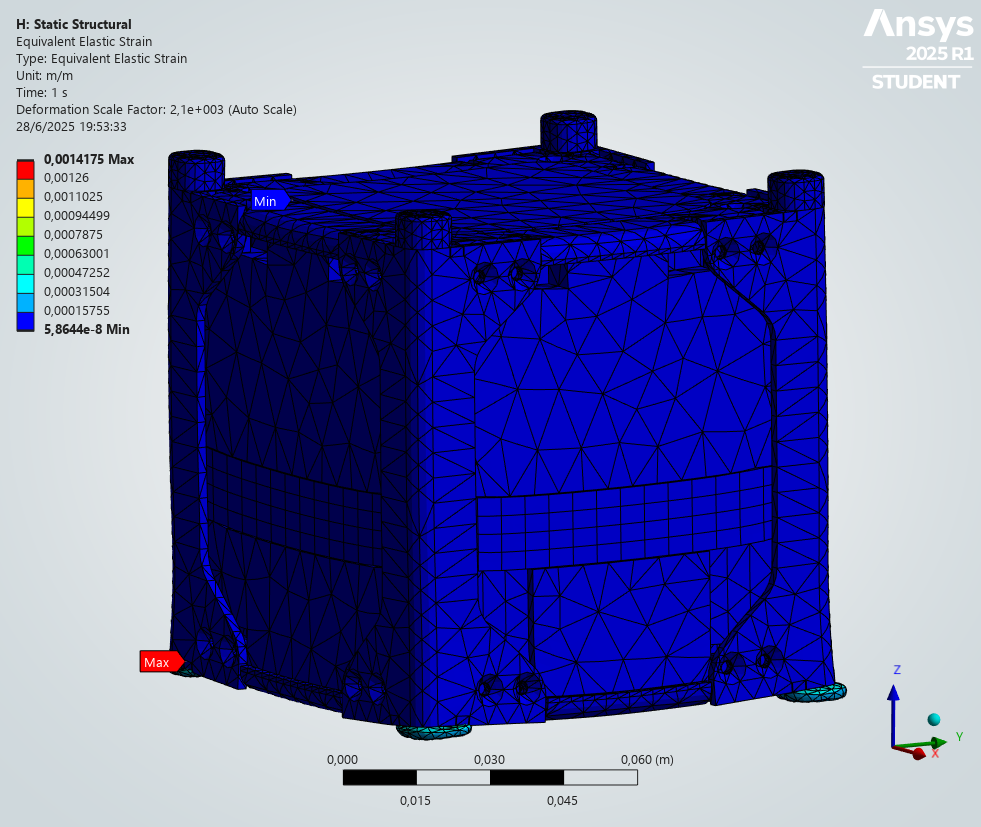
\includegraphics[width=\textwidth]{image/fem/ansys_cubesat-static_strain.png}
          \caption{Análisis de tensión}
          \label{fig:fem_static_strain}
        \end{minipage}
        \begin{minipage}{0.5\textwidth}
          \centering
          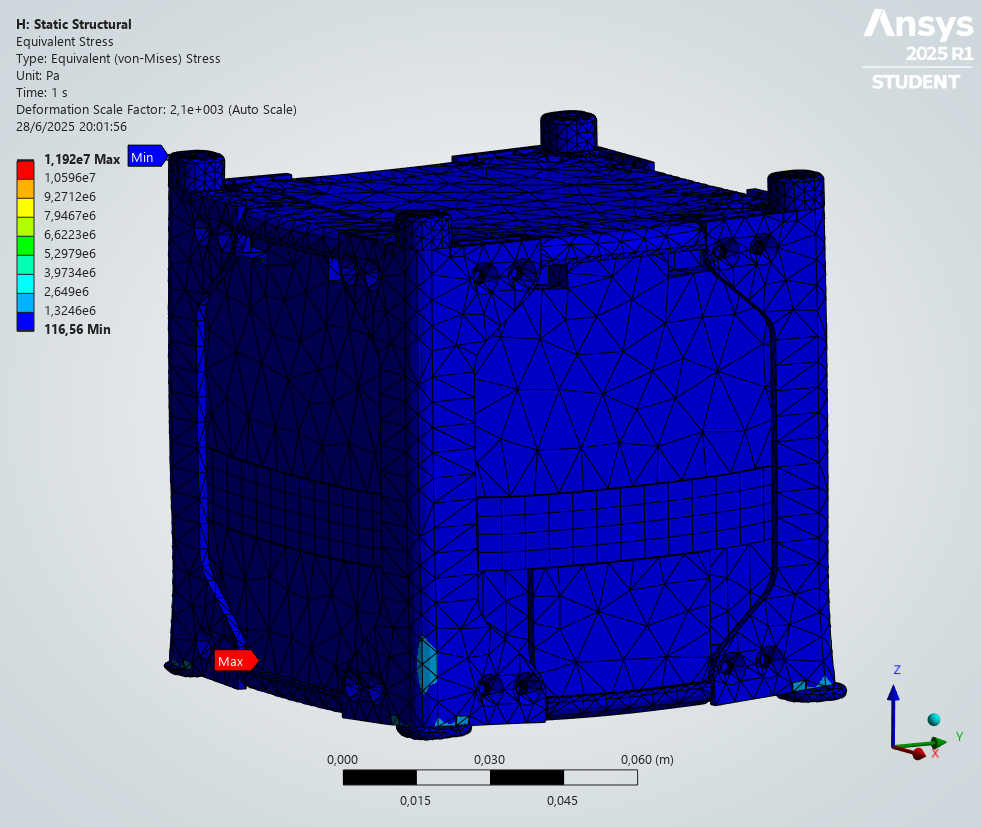
\includegraphics[width=\textwidth]{image/fem/ansys_cubesat-static_stress.png}
          \caption{Análisis de estrés}
          \label{fig:fem_static_stress}
        \end{minipage}
      \end{figure}
      \begin{figure}[H]
        \begin{minipage}{0.5\textwidth}
          \centering
          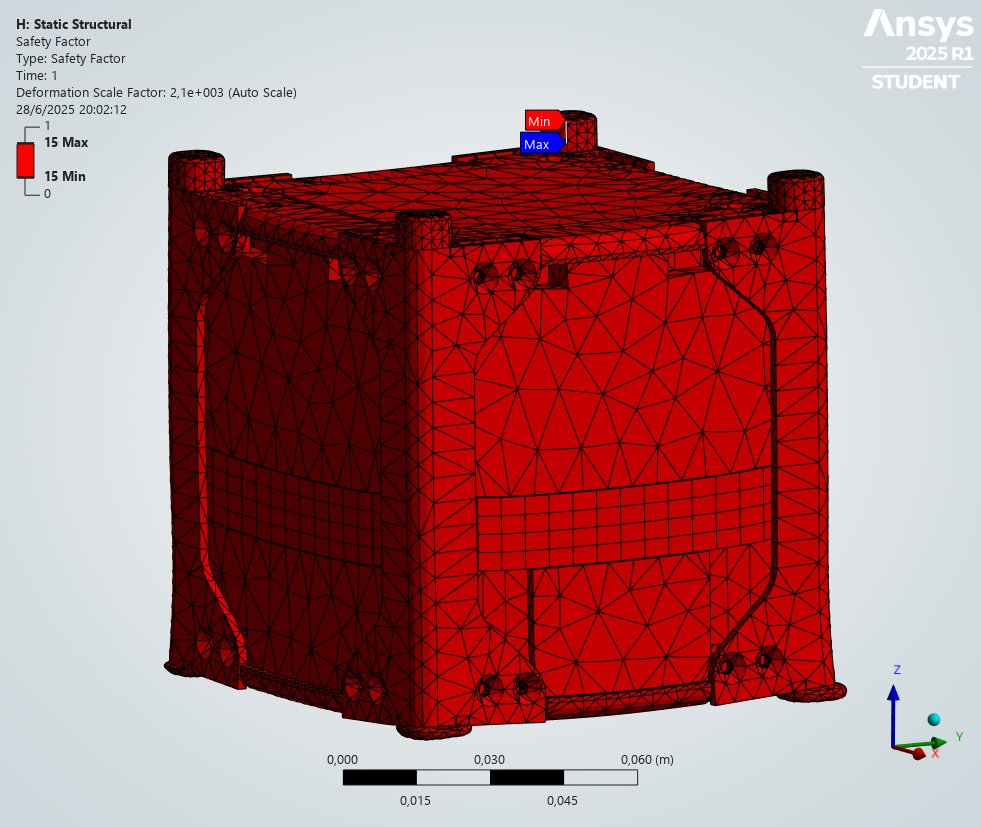
\includegraphics[width=\textwidth]{image/fem/ansys_cubesat-static_safety.png}
          \caption{Análisis de factor de seguridad}
          \label{fig:fem_static_safety}
        \end{minipage}
        \begin{minipage}{0.5\textwidth}
          \centering
          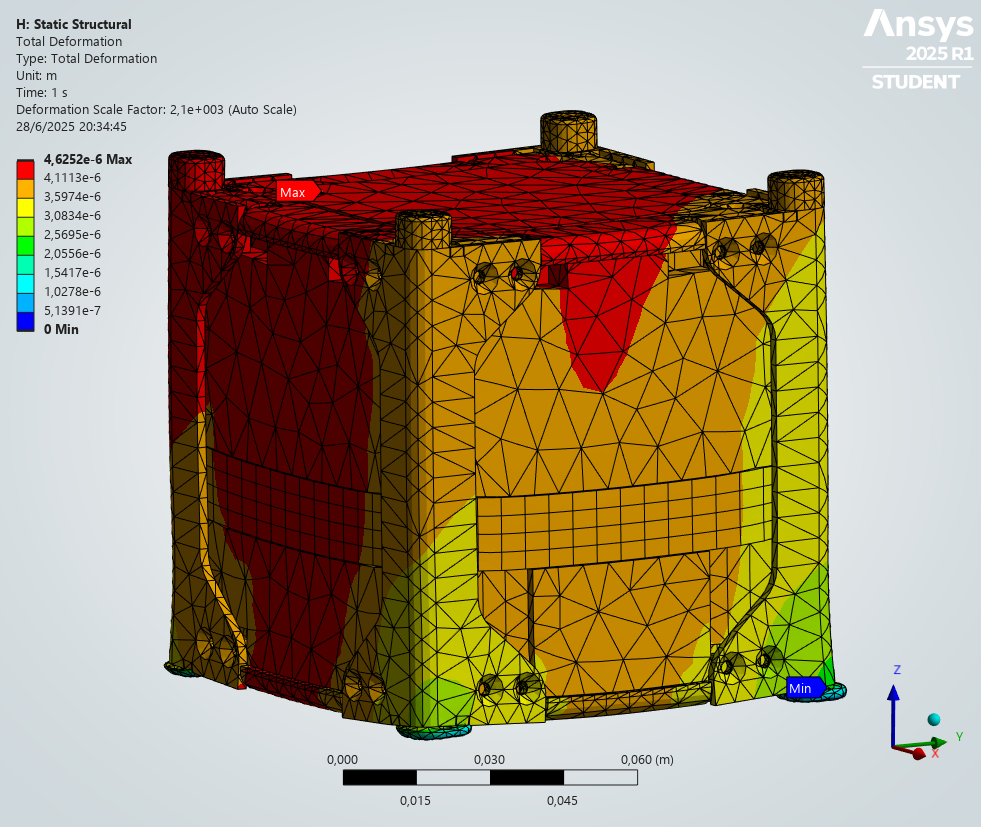
\includegraphics[width=\textwidth]{image/fem/ansys_cubesat-static_deformation.png}
          \caption{Análisis de deformación total}
          \label{fig:fem_static_deformation}
        \end{minipage}
      \end{figure}

      Como se observa en la figura \ref{fig:fem_static_strain}, la tensión máxima alcanzada en la estructura es de
      $19.106 \, Pa$, valor significativamente inferior al limite de rotura del material, lo que indica que no existe
      riesgo estructural bajo las condiciones de carga previstas para el lanzamiento. Asimismo, la figura
      \ref{fig:fem_static_safety} muestra que el factor de seguridad es uniforme en toda la estructura y alcanza un
      valor constante de 15, lo cual proporciona un amplio margen respecto a posibles fallos. Finalmente, según la
      figura \ref{fig:fem_static_deformation}, la deformación máxima experimentada por el CubeSat es de apenas $4\um$,
      lo cual resulta despreciable frente a las tolerancias mecánicas del sistema.

      Concluimos entonces que nuestra propuesta de estructura es valida y soportara las condiciones de lanzamiento.

  \subsection{Análisis de Riesgos}
    En esta sección se identifican posibles fallos asociados al funcionamiento de los subsistemas
    del CubeSat, con el objetivo de implementar estrategias de mitigación que contribuyan a
    aumentar la confiabilidad y la seguridad del sistema en cada fase de la misión. Identificación:

    \begin{longtable}{ | m{2.5cm} | m{3cm} | m{3cm} | m{6cm} | }
      \caption{Análisis de Riesgos} \label{tab:analisis_riesgos} \\
      \hline
      \textbf{Riesgo} & \textbf{Causa} & \textbf{Impacto} & \textbf{Mitigación} \\
      \hline
      \endfirsthead

      \hline
      \textbf{Riesgo} & \textbf{Causa} & \textbf{Impacto} & \textbf{Mitigación} \\
      \hline
      \endhead

      \hline
      \endfoot

      \hline
      \endlastfoot

      Rotura de cápsulas de muestras & Sobrecargas mecánicas o vibraciones excesivas & Pérdida parcial o total de las muestras biológicas & Diseño de porta-cápsulas amortiguadoras. Pruebas de vibración según estándar GEVS. Cierre redundante de las tapas. \\
      \hline
      Fallo del sistema de regulación térmica & Mal dimensionamiento de los elementos Peltier o fallo de controlador en vuelo. & Exposición de muestras a temperaturas fuera de rango. & Control de temperatura con sensores. Validación térmica en cámara climática. Modos de degradación segura que desactivan los elementos Peltier para reducir consumo. \\
      \hline
      Pérdida de datos por fallo de almacenamiento & Corrupción de tarjeta microSD o falla en conmutación RAID por script. & Pérdida parcial o total de registros de muestras. & Verificación periódica de integridad (checksum SHA-256). Script de conmutación automática probado en \acrshort{pdr}. Redundancia de almacenamiento de datos críticos. \\
      \hline
      Fallo del suministro eléctrico & Sobrecarga de rieles, cortocircuito o desconexión no deseada. & Apagado de subsistemas. & Protección contra sobre-corriente y subtensión en \acrshort{pms}. Pruebas de ciclos de carga-descarga de batería. Rieles críticos alimentados desde canales independientes. \\
      \hline
      Mal funcionamiento de la \acrshort{imu} o barómetro & Descalibración por choque mecánico o ruido eléctrico. & Imposibilidad de determinar fases de vuelo con precisión. & Pruebas previas en condiciones similares. \\
      \hline
      Contaminación o degradación de muestras biológicas & Fugas de medios de cultivo, exposición al ambiente. & Resultados experimentales no válidos, pérdida de muestras. & Sellado hermético de tubos. Uso de materiales biocompatibles. Control de humedad en bahía de muestras. Análisis de vacío. \\
      \hline
      Fallo de comunicación pre lanzamiento y pos lanzamiento  & Rotura de hardware por aterrizaje o vuelo. & Imposibilidad de monitoreo inmediato luego del lanzamiento. & Conexión por UART. \\
      \hline
    \end{longtable}

  \subsection{Ensayos}
    En esta sección se detallan los ensayos que se realizarán a los distintos prototipos que surgirán durante el
    desarrollo del CubeSat, que servirán para validar y obtener una retroalimentación del proceso de diseño.

    Sobre el producto final se realzaran ensayos mas exhaustivos que serán detallados en el \acrshort{cdr}.

    \subsubsection{Estructura}
      Para determinar la integridad estructural se realizarán distintos tipos de pruebas, donde las condiciones de cada
      una serán acordes a las del lanzamiento, y también se realizarán pruebas extremas, para encontrar los limites de
      la estructura y poder ampliar el margen de seguridad. Para lograr esto, se realizarán varias estructuras, y se las
      rellenará con subsistemas vacíos pero con el peso necesario para llegar al régimen.

      Las pruebas que se realizarán a la estructura son:
      \begin{itemize}
        \item Prueba de vibraciones: Se somete el prototipo a una cama de vibraciones para determinar si se mantiene en
          forma durante todo el rango de frecuencias y mas.
        \item Prueba de caída: Se somete el prototipo a pruebas de caída de diferentes alturas y buscando que impacte en
          diferentes puntos de la estructura para probar la rigidez estructural y capacidad de contención de las
          carcasas de los subsistemas.
        \item Prueba de fuerzas: Se somete el prototipo a fuerzas (que ingresan y egresan a la estructura) ejercidas en
          puntos críticos donde las tensiones pueden alcanzar picos y generar deformaciones.
      \end{itemize}
    \subsubsection{Peso}
      Para determinar que el CubeSat se encuentra dentro del régimen, a medida que se vayan haciendo los diferentes
      prototipos se pesará todo el CubeSat que se tenga hasta el momento para tener estimaciones mas precisas de peso, y
      poder llegar con el margen de tolerancias especificado sin tener que hacer cambios grandes.

    \subsubsection{Centro de masa}
      Para determinar experimentalmente el centro de masa del CubeSat, colocamos una madera rectangular de espesor
      mínimo sobre una superficie plana de modo que el lado mas estrecho y largo se encuentre en contacto con la
      superficie. Arriba colocamos el CubeSat formando 4 ángulos rectos, es decir que las direcciones sus aristas sean
      paralelas y perpendiculares a la dirección de la madera. Deslizamos el CubeSat horizontalmente hasta encontrar un
      punto de equilibrio, esa será la coordenada del centro de masa en ese eje. Repetimos el procedimiento para los
      demás ejes y verificamos, en cada caso, que se encuentren a una distancia del centro geométrico de a lo sumo 10
      mm.

    \subsubsection{Baterías}
      \begin{itemize}
        \item \textbf{Capacidad real:} este ensayo tiene como finalidad determinar la capacidad efectiva de la batería,
          comparándola con la especificación nominal del fabricante. Para ello, se descargará la batería con una
          corriente constante conocida hasta alcanzar el voltaje mínimo especificado. Se registrará el tiempo total de
          descarga para calcular la capacidad en mAh.  El resultado permitirá verificar si la batería puede sostener la
          demanda energética del sistema durante el tiempo requerido.

        \item \textbf{Medición de voltaje y corriente durante carga y descarga:} Durante las fases de carga y descarga,
          se monitorearan de forma continua los valores de tensión y corriente entregados por la batería. Esto permitirá
          evaluar la estabilidad de las baterias frente a distintas condiciones de carga, asi como detectar cadas de tensión
          o comportamientos no deseados que puedan comprometer la operación de los subsistemas.

        \item \textbf{Medición de temperatura:} durante los ensayos anteriores se registrará también la evolución
          térmica de la batería. Esto permitirá identificar posibles sobrecalentamientos que puedan comprometer la
          seguridad o el rendimiento del sistema.
      \end{itemize}

\section{Plan de Proyecto}

  \subsection{General}
    Para llevar a cabo la misión del CubeSat, se ha definido una estructura de trabajo que
    divide al equipo en diferentes grupos, cada uno con responsabilidades especificas. Esta división
    busca optimizar el desarrollo del proyecto mediante una organización eficiente de tareas y
    recursos humanos.
    \subsubsection{Organización del Equipo}
      \begin{itemize}
        \item \textbf{Project Manager (PM)}
          Coordinador general del proyecto, responsable de la planificación y del funcionamiento
          sincronizado de todos los grupos y subsistemas.
          \begin{itemize}
            \item Cortesini Perez, Luciano Tomas
          \end{itemize}
        \item \textbf{Grupo Mecánico}
         Encargado del diseño estructural del CubeSat.
          \begin{itemize}
            \item Cortesini Perez, Luciano Tomas
            \item Palombo, Franco
          \end{itemize}
        \item \textbf{Grupo Electrónica}
          Responsable del diseño, desarrollo y pruebas de los subsistemas electrónicos, incluyendo
          potencia y sensores.
          \begin{itemize}
            \item Gil, Ignacio
            \item Prieto, Angelo
          \end{itemize}
          \item \textbf{Grupo Software}
          Encargado del desarrollo del software tanto embarcado como de recuperación y procesamiento de datos.
          \begin{itemize}
            \item Adragna, Jimena Sofa
            \item Koroch, Matias Adolfo
            \item Montesinos, Dana Carolina
          \end{itemize}
        \item \textbf{Grupo de Divulgación}
          A medida de que nos interiorizábamos mas con nuestra misión e interactuábamos con
          distintos profesionales, docentes e instituciones que nos brindaron su tiempo y conocimiento
          como equipo nos empezamos a preguntar, de que manera podemos utilizar
          nuestro proyecto para impactar el la sociedad?

          Es así como nace el grupo de Divulgación para darle respuesta a una inquietud que
          surgió fruto del desarrollo de este proyecto. Consideramos valioso compartir los trabajos
          que se llevan a cabo en nuestra facultad para visibilizar el trabajo académico, motivar
          a otros estudiantes, reconocer el valor de la investigación científica como as también
          crear puentes entre la universidad y la sociedad. No solo buscamos cumplir con los
          objetivos técnicos y científicos de la misión, sino también inspirar y promover el interés
          por la ciencia en la comunidad de nuestra región.

          Es por esto que designamos un grupo encargado de documentar las distintas etapas
          del proyecto registrando con fotos y vídeos, generando informes y difundiendo hacia la
          comunidad por medio de distintas plataformas y redes sociales.

          La implementación del plan de comunicación se desarrollara en dos fases. En una primer
          instancia se evaluaran y establecerán los canales digitales y, para ellos, se crearan los
          distintos perfiles institucionales con una identidad unificada en un marco educativo
          y de divulgación científica. Luego, el trabajo se basara en un proceso iterativo en el
          que se documentara sistemáticamente, se editara y adaptara el material multimedia y
          calendario de publicación programada, se realizarán las publicaciones pertinentes y se
          realizara un monitoreo y ajuste basado en la retroalimentación de la comunidad.

          Estimamos no solo llegar a las personas sino también generar dialogo que sea fructífero
          tanto para los demás como para el equipo, debido a esto planeamos ademas adaptar el
          contenido según los intereses del publico, reconocer sus contribuciones e incluir
          herramientas que nos faciliten esta comunicación bidireccional como formatos interactivos
          de preguntas y respuestas, encuestas, sesiones en vivo, entre otras.
          Encargados de la documentación y difusión en el proyecto.
          \begin{itemize}
            \item Adragna, Jimena Sofía
            \item Koroch, Matas Adolfo
            \item Montesinos, Dana Carolina
            \item Prieto, Angelo
          \end{itemize}
      \end{itemize}

  \subsection{Estrategia de documentación y divulgación}

    Con el propósito de consolidar la transparencia, fomentar la comunicación científica y
    promover la apropiación social del conocimiento generado por el Proyecto CubeSat LAMBDA, se ha
    proyectado el desarrollo de una plataforma web pública de documentación y divulgación, dirigida
    tanto a la comunidad académica como al público general. Este portal actuará como repositorio
    centralizado de información técnica y divulgativa, posibilitando la consulta interactiva, el
    seguimiento del progreso de la misión y el acceso a documentación validada.

    \subsubsection{Estructura y contenidos propuestos}

    La plataforma será concebida con una arquitectura modular, atendiendo a criterios de
    accesibilidad universal y facilidad de actualización. Las secciones propuestas
    comprenden:

    \begin{itemize}

      \item Inicio: introducción concisa al proyecto, con enlaces destacados a secciones relevantes.

      \item La misión: exposición de los objetivos científicos y tecnológicos, marco institucional y
      colaboraciones estratégicas (INIMEC-CONICET-UNC).

      \item Cronograma y estado de avance: representación gráfica interactiva del cronograma del proyecto,
      destacando etapas concluidas y próximas actividades.

      \item El equipo: presentación del equipo multidisciplinario, incluyendo roles, funciones y perfiles
      académicos.

      \item Documentación técnica: acceso público a documentos (PDR, PDU, CDR, informes de verificación),
      diagramas, manuales y diseños de interfaz, acompañados de mecanismos de control de versiones y trazabilidad.

      \item Datos abiertos: visualización dinámica y descarga de los datos recolectados por el CubeSat 
      presión, aceleración, temperatura, etc.), disponibles en formatos estandarizados, junto con la
      documentación.

      \item Divulgación científica: materiales didácticos adaptados a diversos niveles
      educativos.

      \item Interacción y comunidad: espacios de comunicación con el público (formularios de contacto,
      sección de preguntas frecuentes, suscripciones a boletines y foros de discusión).
    \end{itemize}

      \subsubsection{Consideraciones técnicas}

    El diseño de la plataforma garantizará el cumplimiento de estándares de accesibilidad, así como
    su adaptación a diversos dispositivos y navegadores. Se implementará una arquitectura desacoplada
    y escalable, utilizando para la capa de servidor.

    Se priorizarán atributos como la seguridad (encriptación HTTPS), alta disponibilidad y versionado
    robusto del contenido.


  \subsection{Cronograma}
    Con el objetivo de garantizar una ejecución ordenada, eficiente y dentro de los plazos
    establecidos, se elaboro un cronograma detallado para cada uno de los grupos de trabajo que
    contempla las diferentes tareas ha realizar junto con los diferentes fechas y plazos estipulados
    para cada una de ellas.

    Utilizamos una herramienta basada en diagramas Gantt de gestión estratégica para lograr
    visualizar con facilidad la secuencia lógica de actividades, sus respectivas duraciones, y las
    dependencias entre tareas.

    Para el desarrollo de este proceso se tuvieron en cuenta distintas variables como las fechas
    limites, los objetivos planteados, la disponibilidad de tiempo, los recursos económicos y el
    capital humano.

    \subsubsection{Grupo Mecánico}
    Para una visualización del cronograma, se remite al diagrama Gantt incluido en el anexo, figura
    \ref{gantt-mecanica1} y figura \ref{gantt-mecanica2}.
    \subsubsection{Grupo Electrónica}
    Para una visualización del cronograma, se remite al diagrama Gantt incluido en el anexo, figura
    \ref{gantt-hardware}.
    \subsubsection{Grupo Software}
    Para una visualización del cronograma, se remite al diagrama Gantt incluido en el anexo.
  \subsection{Costos y Financiamiento}

  La validación de los requisitos funcionales y operacionales del CubeSat requiere la
  disponibilidad de insumos, herramientas, equipamiento e infraestructura adecuada que permitan
  llevar a cabo pruebas técnicas rigurosas. En este sentido, la presente sección contempla la
  financiación necesaria para la adquisición de los materiales e instrumentos que permitan
  fabricar el CubeSat, así como realizar los ensayos pertinentes para el cumplimiento de las especificaciones establecidas.

  La financiación prevista abarca los siguientes componentes:

  \begin{itemize}
    \item \textbf{Adquisición de insumos}: incluye sensores, microcontroladores, estructuras mecánicas, módulos de
      almacenamiento, elementos de conexión y otros componentes electrónicos y estructurales
      necesarios para la fabricación del CubeSat.

    \item \textbf{Herramientas de validación y ensayo}: contempla equipamiento de medición,
      dispositivos de prueba funcional, sistemas de monitoreo térmico y mecánico, así como
      herramientas de ensamblaje y diagnóstico utilizadas durante las etapas de verificación.

    \item \textbf{Acceso a infraestructura y servicios}: incluye la utilización de laboratorios y
      bancos de prueba. En particular, se destaca el acceso a las instalaciones del \textit{Centro de
      Investigación en Informática para la Ingeniería (CIII)} y del \textit{Instituto de
      Investigación Médica Mercedes y Martín Ferreyra (INIMEC-CONICET-UNC)}, los cuales
      proporcionan equipamiento especializado, condiciones técnicas adecuadas y asesoramiento científico
      para la ejecución de los ensayos requeridos.

  \end{itemize}

  Los recursos económicos serán obtenidos a través del respaldo de personas, grupos o
  instituciones interesadas en promover la investigación científica y tecnológica del proyecto.
  Asimismo, se aprovecharán los recursos institucionales disponibles dentro del marco académico.

  Esta estrategia de financiación tiene como objetivo asegurar la disponibilidad de medios
  materiales y técnicos suficientes para cumplir con los planes de verificación y validación
  del satélite, garantizando su operatividad, confiabilidad y compatibilidad con los criterios
  normativos establecidos.

   \begin{table}[H]
     \centering
     \begin{tabular}{|l|r|r|r|}
     \hline
     \textbf{Item} & \textbf{Cantidad} & \textbf{Precio} & \textbf{Subtotal} \\
     \hline
     RPI Zero 2W                            & 1     & 36299  & 36299  \\
     Micro SD 16GB                          & 2     & 13619  & 27238  \\
     Arduino NANO                           & 1     & 6190   & 6190   \\
     Plancha de aluminio 2mm (medio m2)     & 0.25  & 82000  & 20500  \\
     Varillas acero inoxidable 5mm          & 1     & 4900   & 4900   \\
     Baterías LI-PO 3,7V 3200mAh 90x40x4mm   & 5     & 4399   & 21995  \\
     Filamento PP-T grilon3                 & 0.5   & 24780  & 12390  \\
     Placa de cobre virgen 20x10cm          & 1     & 6700   & 6700   \\
     Celda Peltier 30x30mm                  & 3     & 18700  & 56100  \\
     Thermistor ntc 100k                    & 3     & 3890   & 11670  \\
     MPU9250 (\acrshort{imu})               & 1     & 22490  & 22490  \\
     BMP280                                 & 1     & 2344   & 2344   \\
     Componentes electrónicos varios        & 1     & 50000  & 50000  \\
     Tornillería                            & 1     & 20000  & 20000  \\
     \hline
     \multicolumn{3}{|r|}{\textbf{Total:}} & \textbf{298816} \\
     \hline
     \end{tabular}
     \caption{Costos}
     \label{tab:costos}
   \end{table}
